% lecture12.tex -- GENERATED by build_L12.py from L12_numbers.json; do not edit by hand.
\documentclass[10pt,aspectratio=169,t]{beamer}
% =============================================================================
% nn_preamble.tex -- shared Beamer preamble of Neural Networks and Deep Learning (NN)
% Used by every lecture: lectures/Lk/lecturek.tex does
%   \documentclass[10pt,aspectratio=169,t]{beamer}
%   % =============================================================================
% nn_preamble.tex -- shared Beamer preamble of Neural Networks and Deep Learning (NN)
% Used by every lecture: lectures/Lk/lecturek.tex does
%   \documentclass[10pt,aspectratio=169,t]{beamer}
%   % =============================================================================
% nn_preamble.tex -- shared Beamer preamble of Neural Networks and Deep Learning (NN)
% Used by every lecture: lectures/Lk/lecturek.tex does
%   \documentclass[10pt,aspectratio=169,t]{beamer}
%   \input{../common/nn_preamble}
%   \nnlecture{k}{Lecture title}
% Logos live in lectures/common/logos/, charts in lectures/Lk/charts/.
% Do NOT add \hfuzz / \vfuzz / \hbadness here: overfull boxes must be fixed, not hidden.
% =============================================================================

\usetheme{default}
\setbeamersize{text margin left=7mm, text margin right=7mm}

% ---------------------------------------------------------------- packages
\usepackage[utf8]{inputenc}
\usepackage[T1]{fontenc}
\usepackage{lmodern}
\usepackage{amsmath, amssymb}
\usepackage{mathtools}
\usepackage{bm}
\usepackage{tikz}
\usetikzlibrary{arrows.meta, positioning, calc, shapes.misc}
\usepackage{booktabs}
\usepackage{array}
\usepackage{graphicx}
\usepackage{colortbl}
\usepackage{xcolor}
\usepackage{multicol}
\hypersetup{colorlinks=true, linkcolor=MainBlue, urlcolor=MainBlue, citecolor=MainBlue}
\graphicspath{{../common/logos/}}   % charts are included with their language folder: charts/en/, charts/ro/

% ---------------------------------------------------------------- colours
\definecolor{MainBlue}{RGB}{26, 58, 110}
\definecolor{IDAred}{RGB}{205, 0, 0}
\definecolor{DarkGray}{RGB}{51, 51, 51}
\definecolor{FooterGray}{RGB}{100, 100, 100}
\definecolor{BlockGray}{RGB}{236, 238, 242}
\definecolor{KeynoteGray}{RGB}{218, 218, 218}
\definecolor{Crimson}{RGB}{190, 40, 50}
\definecolor{Forest}{RGB}{30, 110, 50}
\definecolor{Bitter}{RGB}{214, 150, 20}
% chart palette (same hex values and order as lectures/common/nn_plot.py SERIES)
\definecolor{Ser1}{HTML}{2A78D6}
\definecolor{Ser2}{HTML}{EB6834}
\definecolor{Ser3}{HTML}{1BAF7A}
\definecolor{Ser4}{HTML}{EDA100}
\definecolor{Ser5}{HTML}{E87BA4}
\definecolor{Ser6}{HTML}{008300}
\definecolor{Ser7}{HTML}{6250D6}
\definecolor{Ser8}{HTML}{E34948}

\setbeamertemplate{background}{%
  \begin{tikzpicture}[remember picture, overlay]
    \shade[shading=axis, shading angle=315, top color=white, bottom color=KeynoteGray]
      (current page.south west) rectangle (current page.north east);
  \end{tikzpicture}}
\setbeamercolor{background canvas}{bg=}
\setbeamercolor{structure}{fg=MainBlue}
\setbeamercolor{normal text}{fg=DarkGray}
\setbeamercolor{title}{fg=IDAred}
\setbeamercolor{frametitle}{fg=IDAred, bg=}
\setbeamercolor{block title}{bg=MainBlue, fg=white}
\setbeamercolor{block body}{bg=BlockGray, fg=DarkGray}
\setbeamercolor{block title alerted}{bg=Crimson, fg=white}
\setbeamercolor{block body alerted}{bg=Crimson!7, fg=DarkGray}
\setbeamercolor{block title example}{bg=Forest, fg=white}
\setbeamercolor{block body example}{bg=Forest!7, fg=DarkGray}
\setbeamercolor{item}{fg=MainBlue}
\setbeamerfont{frametitle}{size=\large, series=\bfseries}
\setbeamerfont{block title}{size=\small, series=\bfseries}
\setbeamertemplate{blocks}[rounded][shadow=false]
\setbeamertemplate{itemize item}{\color{MainBlue}$\boxdot$}
\setbeamertemplate{itemize subitem}{\color{MainBlue}\scriptsize$\blacktriangleright$}
% compact two-level lists: level 1 = main point, level 2 = details (no text outside bullets)
\setbeamerfont{itemize/enumerate subbody}{size=\footnotesize}
\setlength{\leftmargini}{1.1em}
\setlength{\leftmarginii}{1.1em}
\setbeamertemplate{itemize/enumerate body begin}{\setlength{\topsep}{0pt}\setlength{\partopsep}{0pt}\setlength{\parskip}{0pt}}
\setbeamertemplate{itemize/enumerate subbody begin}{\setlength{\topsep}{0pt}\setlength{\partopsep}{0pt}\setlength{\itemsep}{0pt}\vspace{-0.4ex}}

\setbeamertemplate{enumerate item}{\color{MainBlue}\insertenumlabel.}
\setlength{\leftmargini}{1.3em}
\setlength{\leftmarginii}{1.2em}
\setbeamertemplate{navigation symbols}{}
\setbeamertemplate{section in toc}{\color{MainBlue}$\blacktriangleright$~\inserttocsection}
\setbeamertemplate{caption}{\raggedright\insertcaption\par}
% frame subtitle = precise citation line under the claim title (Weron style)
\setbeamerfont{framesubtitle}{size=\footnotesize}
\setbeamercolor{framesubtitle}{fg=FooterGray}
% outline that reappears at every section with the current section highlighted
\setbeamertemplate{section in toc shaded}[default][35]
\setbeamertemplate{subsection in toc shaded}[default][35]
\setbeamertemplate{subsection in toc}{\leavevmode\leftskip=2.2em\color{DarkGray}\small\inserttocsubsection\par}
\AtBeginSection[]{{\begin{frame}{\txtoutline}\vspace{2mm}\small
  \tableofcontents[currentsection,hideothersubsections]\end{frame}}}

% ---------------------------------------------------------------- head and foot
\setbeamertemplate{headline}{%
  \vskip10pt%
  \hbox to \paperwidth{\hskip0.5cm%
    {\small\color{FooterGray}\renewcommand{\hyperlink}[2]{##2}\insertsectionhead}%
    \hfill\textcolor{FooterGray}{\small\insertframenumber}\hskip0.5cm}%
  \vskip4pt{\color{FooterGray}\hrule height 0.4pt}}
% footer as in the other courses (MFM, SFM): course name on the left, small sparkline on the right
\setbeamertemplate{footline}{%
  {\color{FooterGray}\hrule height 0.4pt}\vskip4pt%
  \hbox to \paperwidth{\hskip0.5cm%
    \textcolor{FooterGray}{\small\txtcourse}%
    \hfill\raisebox{-0.1em}{\begin{tikzpicture}[x=0.08em, y=0.08em, line width=0.4pt]
      \draw[FooterGray] (0,3) -- (1,4) -- (2,3.5) -- (3,5) -- (4,4) -- (5,6) -- (6,5.5) -- (7,4) -- (8,5) -- (9,7) -- (10,6) -- (11,5) -- (12,6.5) -- (13,8) -- (14,7) -- (15,6) -- (16,7.5) -- (17,9) -- (18,8) -- (19,7) -- (20,8.5) -- (21,10) -- (22,9) -- (23,8) -- (24,9.5);
    \end{tikzpicture}}\hskip0.5cm}%
  \vskip6pt}

% ---------------------------------------------------------------- title page
\defbeamertemplate*{title page}{nn}[1][]{%
  \vspace{0.15cm}
  \begin{center}
    \href{https://www.ase.ro}{
\includegraphics[height=0.9cm]{ase_logo.png}}\hspace{0.3cm}%
    \href{https://ipe.ro/new}{
\includegraphics[height=0.9cm]{acad_logo.png}}\hspace{0.3cm}%
    \href{https://theida.net}{
\includegraphics[height=0.9cm]{ida_logo.png}}\hspace{0.3cm}%
    \href{https://blockchain-research-center.com}{
\includegraphics[height=0.9cm]{brc_logo.png}}\hspace{0.3cm}%
    \href{https://www.ai4efin.ase.ro}{
\includegraphics[height=0.9cm]{ai4efin_logo.png}}\hspace{0.3cm}%
    \href{https://www.digital-finance-msca.com}{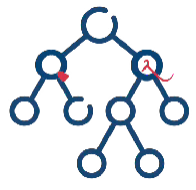
\includegraphics[height=0.9cm]{msca_logo.png}}%
  \end{center}
  \vspace{0.45cm}
  \begin{center}
    \begin{minipage}{0.1\textwidth}\centering
      \href{https://quantlet.com}{
\includegraphics[height=0.9cm]{ql_logo.png}}\end{minipage}%
    \begin{minipage}{0.78\textwidth}\centering
      {\Large\bfseries\usebeamercolor[fg]{title}\inserttitle}\par\vspace{0.25cm}
      {\large\usebeamercolor[fg]{title}\insertsubtitle}\end{minipage}%
    \begin{minipage}{0.1\textwidth}\centering
      \href{https://quantinar.com}{
\includegraphics[height=0.9cm]{qr_logo.png}}\end{minipage}
  \end{center}
  \vfill
  \hspace{0.4cm}{\bfseries\insertauthor}\par\vspace{0.12cm}
  \hspace{0.4cm}\begin{minipage}[t]{0.92\textwidth}\raggedright\footnotesize\insertinstitute\end{minipage}
  \par\vspace{0.4cm}}

% ---------------------------------------------------------------- lecture metadata
\newcommand{\nnshort}{}
\newcommand{\nnnb}{notebooks}
\newcommand{\nnrepo}{https://github.com/danpele/NEURAL_BIZ/tree/main}
% language-dependent labels (English default; \nnromanian switches to Romanian, call it before \nnlecture)
\newcommand{\txtcourse}{Neural Networks and Deep Learning}
\newcommand{\txtlecture}{Lecture}
\newcommand{\txtoutline}{Outline}
\newcommand{\txtintuition}{In one sentence:}
\newcommand{\txtjob}{In practice:}
\newcommand{\txttry}{Experiment yourself:}
\newcommand{\txtwhere}{where}
\newcommand{\txtsim}{SIMULATED DATA (teaching illustration)}
\newcommand{\txtnbsuffix}{}
\newcommand{\txtinstitute}{Bucharest University of Economic Studies (ASE), Department of Statistics and Econometrics\\
    Romanian Academy, Institute for Economic Forecasting (IPE)\\
    IDA Institute Digital Assets \textbullet\ AI4EFin \textbullet\ MSCA Digital Finance}
\newcommand{\nnromanian}{%
  \renewcommand{\txtcourse}{Rețele neuronale și deep learning}%
  \renewcommand{\txtlecture}{Cursul}%
  \renewcommand{\txtoutline}{Cuprins}%
  \renewcommand{\txtintuition}{Pe scurt:}%
  \renewcommand{\txtjob}{În practică:}%
  \renewcommand{\txttry}{Exercițiu practic:}%
  \renewcommand{\txtwhere}{unde}%
  \renewcommand{\txtsim}{DATE SIMULATE (doar pentru ilustrare)}%
  \renewcommand{\txtnbsuffix}{\string_ro}%
  \renewcommand{\txtinstitute}{Academia de Studii Economice din București (ASE), Departamentul de Statistică și Econometrie\\
    Academia Română, Institutul de Prognoză Economică (IPE)\\
    IDA Institute Digital Assets \textbullet\ AI4EFin \textbullet\ MSCA Digital Finance}}
\newcommand{\nnlecture}[2]{%
  \renewcommand{\nnshort}{\txtlecture\ #1}%
  \renewcommand{\nnnb}{notebooks/L#1\string_notebook\txtnbsuffix.ipynb}%
  \title[NN]{\txtcourse}%
  \subtitle{\txtlecture\ #1: #2}%
  \author{Prof.\ dr.\ Daniel Traian PELE}%
  \institute{\txtinstitute}%
  \date{}}

% ---------------------------------------------------------------- teaching blocks (one message per frame)
% \intuition{one plain sentence}  ->  formula with every symbol defined  ->  real-data example  ->  \manager{one line}
\newcommand{\intuition}[1]{\begin{itemize}\item {\color{MainBlue}\textbf{\txtintuition}}~#1\end{itemize}\vspace{0.6mm}}
\newcommand{\manager}[1]{\colorbox{Forest!10}{\parbox{\dimexpr\linewidth-2\fboxsep\relax}{\footnotesize
  \begin{itemize}\setlength{\itemsep}{0pt}\item \textbf{\color{Forest}\txtjob}~#1\end{itemize}}}}
% Experiment yourself: pointer to the matching notebook section
\newcommand{\tryit}[1]{{\scriptsize\href{\nnrepo/\nnnb}{%
  \raisebox{-0.15em}{
\includegraphics[height=0.85em]{ql_logo.png}}\,\textbf{\txttry}~\color{MainBlue}#1}}}
% bottom row: manager line (left) + experiment pointer (right), pinned to the bottom of the frame
\newcommand{\bottomrow}[2]{\par\vfill\noindent\begin{minipage}[b]{0.72\linewidth}#1\end{minipage}\hfill
  \begin{minipage}[b]{0.26\linewidth}\raggedleft #2\end{minipage}\par\vspace{0.5mm}}
\newcommand{\where}[1]{{\footnotesize\textbf{\txtwhere}~#1\par}}

% ---------------------------------------------------------------- helpers
% chart source line under a figure: \chartsource{Source ...; period ...}
\newcommand{\chartsource}[1]{\par\vspace{1pt}{\scriptsize\color{FooterGray}#1\par}}
% link to code: \quantlet{label}{path inside the repo}
\newcommand{\quantlet}[2]{\par\vspace{1pt}\hfill\href{\nnrepo/#2}{%
  \raisebox{-0.15em}{
\includegraphics[height=0.75em]{ql_logo.png}}\textcolor{MainBlue}{\scriptsize\ #1}}}
% inline Quantlet link for the bottom-right corner of a frame: \qlink{label}{path inside the repo}
\newcommand{\qlink}[2]{{\scriptsize\href{\nnrepo/#2}{\raisebox{-0.15em}{
\includegraphics[height=0.85em]{ql_logo.png}}\,\textcolor{MainBlue}{#1}}}}
\newcommand{\simlabel}{\colorbox{Crimson!12}{\scriptsize\bfseries\color{Crimson}\txtsim}}
\newcommand{\E}{\mathbb{E}}
\newcommand{\Var}{\operatorname{Var}}
\newcommand{\Cov}{\operatorname{Cov}}
\newcommand{\Corr}{\operatorname{Corr}}
\newcommand{\asinh}{\operatorname{asinh}}
\newcommand{\iid}{\overset{\text{i.i.d.}}{\sim}}
\newcommand{\EUR}{EUR}
% deep-learning notation (Bishop & Bishop, 2024): vectors bold lower case, matrices bold upper case
\newcommand{\R}{\mathbb{R}}
\newcommand{\vx}{\mathbf{x}}
\newcommand{\vy}{\mathbf{y}}
\newcommand{\vz}{\mathbf{z}}
\newcommand{\vh}{\mathbf{h}}
\newcommand{\vw}{\mathbf{w}}
\newcommand{\vb}{\mathbf{b}}
\newcommand{\mW}{\mathbf{W}}
\newcommand{\mX}{\mathbf{X}}
\newcommand{\btheta}{\boldsymbol{\theta}}
\newcommand{\loss}{\mathcal{L}}
\newcommand{\dataset}{\mathcal{D}}
\DeclareMathOperator*{\argmin}{arg\,min}
\DeclareMathOperator*{\argmax}{arg\,max}
\DeclareMathOperator{\softmax}{softmax}
\DeclareMathOperator{\ReLU}{ReLU}
\DeclareMathOperator{\sigm}{\sigma}

%   \nnlecture{k}{Lecture title}
% Logos live in lectures/common/logos/, charts in lectures/Lk/charts/.
% Do NOT add \hfuzz / \vfuzz / \hbadness here: overfull boxes must be fixed, not hidden.
% =============================================================================

\usetheme{default}
\setbeamersize{text margin left=7mm, text margin right=7mm}

% ---------------------------------------------------------------- packages
\usepackage[utf8]{inputenc}
\usepackage[T1]{fontenc}
\usepackage{lmodern}
\usepackage{amsmath, amssymb}
\usepackage{mathtools}
\usepackage{bm}
\usepackage{tikz}
\usetikzlibrary{arrows.meta, positioning, calc, shapes.misc}
\usepackage{booktabs}
\usepackage{array}
\usepackage{graphicx}
\usepackage{colortbl}
\usepackage{xcolor}
\usepackage{multicol}
\hypersetup{colorlinks=true, linkcolor=MainBlue, urlcolor=MainBlue, citecolor=MainBlue}
\graphicspath{{../common/logos/}}   % charts are included with their language folder: charts/en/, charts/ro/

% ---------------------------------------------------------------- colours
\definecolor{MainBlue}{RGB}{26, 58, 110}
\definecolor{IDAred}{RGB}{205, 0, 0}
\definecolor{DarkGray}{RGB}{51, 51, 51}
\definecolor{FooterGray}{RGB}{100, 100, 100}
\definecolor{BlockGray}{RGB}{236, 238, 242}
\definecolor{KeynoteGray}{RGB}{218, 218, 218}
\definecolor{Crimson}{RGB}{190, 40, 50}
\definecolor{Forest}{RGB}{30, 110, 50}
\definecolor{Bitter}{RGB}{214, 150, 20}
% chart palette (same hex values and order as lectures/common/nn_plot.py SERIES)
\definecolor{Ser1}{HTML}{2A78D6}
\definecolor{Ser2}{HTML}{EB6834}
\definecolor{Ser3}{HTML}{1BAF7A}
\definecolor{Ser4}{HTML}{EDA100}
\definecolor{Ser5}{HTML}{E87BA4}
\definecolor{Ser6}{HTML}{008300}
\definecolor{Ser7}{HTML}{6250D6}
\definecolor{Ser8}{HTML}{E34948}

\setbeamertemplate{background}{%
  \begin{tikzpicture}[remember picture, overlay]
    \shade[shading=axis, shading angle=315, top color=white, bottom color=KeynoteGray]
      (current page.south west) rectangle (current page.north east);
  \end{tikzpicture}}
\setbeamercolor{background canvas}{bg=}
\setbeamercolor{structure}{fg=MainBlue}
\setbeamercolor{normal text}{fg=DarkGray}
\setbeamercolor{title}{fg=IDAred}
\setbeamercolor{frametitle}{fg=IDAred, bg=}
\setbeamercolor{block title}{bg=MainBlue, fg=white}
\setbeamercolor{block body}{bg=BlockGray, fg=DarkGray}
\setbeamercolor{block title alerted}{bg=Crimson, fg=white}
\setbeamercolor{block body alerted}{bg=Crimson!7, fg=DarkGray}
\setbeamercolor{block title example}{bg=Forest, fg=white}
\setbeamercolor{block body example}{bg=Forest!7, fg=DarkGray}
\setbeamercolor{item}{fg=MainBlue}
\setbeamerfont{frametitle}{size=\large, series=\bfseries}
\setbeamerfont{block title}{size=\small, series=\bfseries}
\setbeamertemplate{blocks}[rounded][shadow=false]
\setbeamertemplate{itemize item}{\color{MainBlue}$\boxdot$}
\setbeamertemplate{itemize subitem}{\color{MainBlue}\scriptsize$\blacktriangleright$}
% compact two-level lists: level 1 = main point, level 2 = details (no text outside bullets)
\setbeamerfont{itemize/enumerate subbody}{size=\footnotesize}
\setlength{\leftmargini}{1.1em}
\setlength{\leftmarginii}{1.1em}
\setbeamertemplate{itemize/enumerate body begin}{\setlength{\topsep}{0pt}\setlength{\partopsep}{0pt}\setlength{\parskip}{0pt}}
\setbeamertemplate{itemize/enumerate subbody begin}{\setlength{\topsep}{0pt}\setlength{\partopsep}{0pt}\setlength{\itemsep}{0pt}\vspace{-0.4ex}}

\setbeamertemplate{enumerate item}{\color{MainBlue}\insertenumlabel.}
\setlength{\leftmargini}{1.3em}
\setlength{\leftmarginii}{1.2em}
\setbeamertemplate{navigation symbols}{}
\setbeamertemplate{section in toc}{\color{MainBlue}$\blacktriangleright$~\inserttocsection}
\setbeamertemplate{caption}{\raggedright\insertcaption\par}
% frame subtitle = precise citation line under the claim title (Weron style)
\setbeamerfont{framesubtitle}{size=\footnotesize}
\setbeamercolor{framesubtitle}{fg=FooterGray}
% outline that reappears at every section with the current section highlighted
\setbeamertemplate{section in toc shaded}[default][35]
\setbeamertemplate{subsection in toc shaded}[default][35]
\setbeamertemplate{subsection in toc}{\leavevmode\leftskip=2.2em\color{DarkGray}\small\inserttocsubsection\par}
\AtBeginSection[]{{\begin{frame}{\txtoutline}\vspace{2mm}\small
  \tableofcontents[currentsection,hideothersubsections]\end{frame}}}

% ---------------------------------------------------------------- head and foot
\setbeamertemplate{headline}{%
  \vskip10pt%
  \hbox to \paperwidth{\hskip0.5cm%
    {\small\color{FooterGray}\renewcommand{\hyperlink}[2]{##2}\insertsectionhead}%
    \hfill\textcolor{FooterGray}{\small\insertframenumber}\hskip0.5cm}%
  \vskip4pt{\color{FooterGray}\hrule height 0.4pt}}
% footer as in the other courses (MFM, SFM): course name on the left, small sparkline on the right
\setbeamertemplate{footline}{%
  {\color{FooterGray}\hrule height 0.4pt}\vskip4pt%
  \hbox to \paperwidth{\hskip0.5cm%
    \textcolor{FooterGray}{\small\txtcourse}%
    \hfill\raisebox{-0.1em}{\begin{tikzpicture}[x=0.08em, y=0.08em, line width=0.4pt]
      \draw[FooterGray] (0,3) -- (1,4) -- (2,3.5) -- (3,5) -- (4,4) -- (5,6) -- (6,5.5) -- (7,4) -- (8,5) -- (9,7) -- (10,6) -- (11,5) -- (12,6.5) -- (13,8) -- (14,7) -- (15,6) -- (16,7.5) -- (17,9) -- (18,8) -- (19,7) -- (20,8.5) -- (21,10) -- (22,9) -- (23,8) -- (24,9.5);
    \end{tikzpicture}}\hskip0.5cm}%
  \vskip6pt}

% ---------------------------------------------------------------- title page
\defbeamertemplate*{title page}{nn}[1][]{%
  \vspace{0.15cm}
  \begin{center}
    \href{https://www.ase.ro}{
\includegraphics[height=0.9cm]{ase_logo.png}}\hspace{0.3cm}%
    \href{https://ipe.ro/new}{
\includegraphics[height=0.9cm]{acad_logo.png}}\hspace{0.3cm}%
    \href{https://theida.net}{
\includegraphics[height=0.9cm]{ida_logo.png}}\hspace{0.3cm}%
    \href{https://blockchain-research-center.com}{
\includegraphics[height=0.9cm]{brc_logo.png}}\hspace{0.3cm}%
    \href{https://www.ai4efin.ase.ro}{
\includegraphics[height=0.9cm]{ai4efin_logo.png}}\hspace{0.3cm}%
    \href{https://www.digital-finance-msca.com}{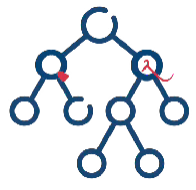
\includegraphics[height=0.9cm]{msca_logo.png}}%
  \end{center}
  \vspace{0.45cm}
  \begin{center}
    \begin{minipage}{0.1\textwidth}\centering
      \href{https://quantlet.com}{
\includegraphics[height=0.9cm]{ql_logo.png}}\end{minipage}%
    \begin{minipage}{0.78\textwidth}\centering
      {\Large\bfseries\usebeamercolor[fg]{title}\inserttitle}\par\vspace{0.25cm}
      {\large\usebeamercolor[fg]{title}\insertsubtitle}\end{minipage}%
    \begin{minipage}{0.1\textwidth}\centering
      \href{https://quantinar.com}{
\includegraphics[height=0.9cm]{qr_logo.png}}\end{minipage}
  \end{center}
  \vfill
  \hspace{0.4cm}{\bfseries\insertauthor}\par\vspace{0.12cm}
  \hspace{0.4cm}\begin{minipage}[t]{0.92\textwidth}\raggedright\footnotesize\insertinstitute\end{minipage}
  \par\vspace{0.4cm}}

% ---------------------------------------------------------------- lecture metadata
\newcommand{\nnshort}{}
\newcommand{\nnnb}{notebooks}
\newcommand{\nnrepo}{https://github.com/danpele/NEURAL_BIZ/tree/main}
% language-dependent labels (English default; \nnromanian switches to Romanian, call it before \nnlecture)
\newcommand{\txtcourse}{Neural Networks and Deep Learning}
\newcommand{\txtlecture}{Lecture}
\newcommand{\txtoutline}{Outline}
\newcommand{\txtintuition}{In one sentence:}
\newcommand{\txtjob}{In practice:}
\newcommand{\txttry}{Experiment yourself:}
\newcommand{\txtwhere}{where}
\newcommand{\txtsim}{SIMULATED DATA (teaching illustration)}
\newcommand{\txtnbsuffix}{}
\newcommand{\txtinstitute}{Bucharest University of Economic Studies (ASE), Department of Statistics and Econometrics\\
    Romanian Academy, Institute for Economic Forecasting (IPE)\\
    IDA Institute Digital Assets \textbullet\ AI4EFin \textbullet\ MSCA Digital Finance}
\newcommand{\nnromanian}{%
  \renewcommand{\txtcourse}{Rețele neuronale și deep learning}%
  \renewcommand{\txtlecture}{Cursul}%
  \renewcommand{\txtoutline}{Cuprins}%
  \renewcommand{\txtintuition}{Pe scurt:}%
  \renewcommand{\txtjob}{În practică:}%
  \renewcommand{\txttry}{Exercițiu practic:}%
  \renewcommand{\txtwhere}{unde}%
  \renewcommand{\txtsim}{DATE SIMULATE (doar pentru ilustrare)}%
  \renewcommand{\txtnbsuffix}{\string_ro}%
  \renewcommand{\txtinstitute}{Academia de Studii Economice din București (ASE), Departamentul de Statistică și Econometrie\\
    Academia Română, Institutul de Prognoză Economică (IPE)\\
    IDA Institute Digital Assets \textbullet\ AI4EFin \textbullet\ MSCA Digital Finance}}
\newcommand{\nnlecture}[2]{%
  \renewcommand{\nnshort}{\txtlecture\ #1}%
  \renewcommand{\nnnb}{notebooks/L#1\string_notebook\txtnbsuffix.ipynb}%
  \title[NN]{\txtcourse}%
  \subtitle{\txtlecture\ #1: #2}%
  \author{Prof.\ dr.\ Daniel Traian PELE}%
  \institute{\txtinstitute}%
  \date{}}

% ---------------------------------------------------------------- teaching blocks (one message per frame)
% \intuition{one plain sentence}  ->  formula with every symbol defined  ->  real-data example  ->  \manager{one line}
\newcommand{\intuition}[1]{\begin{itemize}\item {\color{MainBlue}\textbf{\txtintuition}}~#1\end{itemize}\vspace{0.6mm}}
\newcommand{\manager}[1]{\colorbox{Forest!10}{\parbox{\dimexpr\linewidth-2\fboxsep\relax}{\footnotesize
  \begin{itemize}\setlength{\itemsep}{0pt}\item \textbf{\color{Forest}\txtjob}~#1\end{itemize}}}}
% Experiment yourself: pointer to the matching notebook section
\newcommand{\tryit}[1]{{\scriptsize\href{\nnrepo/\nnnb}{%
  \raisebox{-0.15em}{
\includegraphics[height=0.85em]{ql_logo.png}}\,\textbf{\txttry}~\color{MainBlue}#1}}}
% bottom row: manager line (left) + experiment pointer (right), pinned to the bottom of the frame
\newcommand{\bottomrow}[2]{\par\vfill\noindent\begin{minipage}[b]{0.72\linewidth}#1\end{minipage}\hfill
  \begin{minipage}[b]{0.26\linewidth}\raggedleft #2\end{minipage}\par\vspace{0.5mm}}
\newcommand{\where}[1]{{\footnotesize\textbf{\txtwhere}~#1\par}}

% ---------------------------------------------------------------- helpers
% chart source line under a figure: \chartsource{Source ...; period ...}
\newcommand{\chartsource}[1]{\par\vspace{1pt}{\scriptsize\color{FooterGray}#1\par}}
% link to code: \quantlet{label}{path inside the repo}
\newcommand{\quantlet}[2]{\par\vspace{1pt}\hfill\href{\nnrepo/#2}{%
  \raisebox{-0.15em}{
\includegraphics[height=0.75em]{ql_logo.png}}\textcolor{MainBlue}{\scriptsize\ #1}}}
% inline Quantlet link for the bottom-right corner of a frame: \qlink{label}{path inside the repo}
\newcommand{\qlink}[2]{{\scriptsize\href{\nnrepo/#2}{\raisebox{-0.15em}{
\includegraphics[height=0.85em]{ql_logo.png}}\,\textcolor{MainBlue}{#1}}}}
\newcommand{\simlabel}{\colorbox{Crimson!12}{\scriptsize\bfseries\color{Crimson}\txtsim}}
\newcommand{\E}{\mathbb{E}}
\newcommand{\Var}{\operatorname{Var}}
\newcommand{\Cov}{\operatorname{Cov}}
\newcommand{\Corr}{\operatorname{Corr}}
\newcommand{\asinh}{\operatorname{asinh}}
\newcommand{\iid}{\overset{\text{i.i.d.}}{\sim}}
\newcommand{\EUR}{EUR}
% deep-learning notation (Bishop & Bishop, 2024): vectors bold lower case, matrices bold upper case
\newcommand{\R}{\mathbb{R}}
\newcommand{\vx}{\mathbf{x}}
\newcommand{\vy}{\mathbf{y}}
\newcommand{\vz}{\mathbf{z}}
\newcommand{\vh}{\mathbf{h}}
\newcommand{\vw}{\mathbf{w}}
\newcommand{\vb}{\mathbf{b}}
\newcommand{\mW}{\mathbf{W}}
\newcommand{\mX}{\mathbf{X}}
\newcommand{\btheta}{\boldsymbol{\theta}}
\newcommand{\loss}{\mathcal{L}}
\newcommand{\dataset}{\mathcal{D}}
\DeclareMathOperator*{\argmin}{arg\,min}
\DeclareMathOperator*{\argmax}{arg\,max}
\DeclareMathOperator{\softmax}{softmax}
\DeclareMathOperator{\ReLU}{ReLU}
\DeclareMathOperator{\sigm}{\sigma}

%   \nnlecture{k}{Lecture title}
% Logos live in lectures/common/logos/, charts in lectures/Lk/charts/.
% Do NOT add \hfuzz / \vfuzz / \hbadness here: overfull boxes must be fixed, not hidden.
% =============================================================================

\usetheme{default}
\setbeamersize{text margin left=7mm, text margin right=7mm}

% ---------------------------------------------------------------- packages
\usepackage[utf8]{inputenc}
\usepackage[T1]{fontenc}
\usepackage{lmodern}
\usepackage{amsmath, amssymb}
\usepackage{mathtools}
\usepackage{bm}
\usepackage{tikz}
\usetikzlibrary{arrows.meta, positioning, calc, shapes.misc}
\usepackage{booktabs}
\usepackage{array}
\usepackage{graphicx}
\usepackage{colortbl}
\usepackage{xcolor}
\usepackage{multicol}
\hypersetup{colorlinks=true, linkcolor=MainBlue, urlcolor=MainBlue, citecolor=MainBlue}
\graphicspath{{../common/logos/}}   % charts are included with their language folder: charts/en/, charts/ro/

% ---------------------------------------------------------------- colours
\definecolor{MainBlue}{RGB}{26, 58, 110}
\definecolor{IDAred}{RGB}{205, 0, 0}
\definecolor{DarkGray}{RGB}{51, 51, 51}
\definecolor{FooterGray}{RGB}{100, 100, 100}
\definecolor{BlockGray}{RGB}{236, 238, 242}
\definecolor{KeynoteGray}{RGB}{218, 218, 218}
\definecolor{Crimson}{RGB}{190, 40, 50}
\definecolor{Forest}{RGB}{30, 110, 50}
\definecolor{Bitter}{RGB}{214, 150, 20}
% chart palette (same hex values and order as lectures/common/nn_plot.py SERIES)
\definecolor{Ser1}{HTML}{2A78D6}
\definecolor{Ser2}{HTML}{EB6834}
\definecolor{Ser3}{HTML}{1BAF7A}
\definecolor{Ser4}{HTML}{EDA100}
\definecolor{Ser5}{HTML}{E87BA4}
\definecolor{Ser6}{HTML}{008300}
\definecolor{Ser7}{HTML}{6250D6}
\definecolor{Ser8}{HTML}{E34948}

\setbeamertemplate{background}{%
  \begin{tikzpicture}[remember picture, overlay]
    \shade[shading=axis, shading angle=315, top color=white, bottom color=KeynoteGray]
      (current page.south west) rectangle (current page.north east);
  \end{tikzpicture}}
\setbeamercolor{background canvas}{bg=}
\setbeamercolor{structure}{fg=MainBlue}
\setbeamercolor{normal text}{fg=DarkGray}
\setbeamercolor{title}{fg=IDAred}
\setbeamercolor{frametitle}{fg=IDAred, bg=}
\setbeamercolor{block title}{bg=MainBlue, fg=white}
\setbeamercolor{block body}{bg=BlockGray, fg=DarkGray}
\setbeamercolor{block title alerted}{bg=Crimson, fg=white}
\setbeamercolor{block body alerted}{bg=Crimson!7, fg=DarkGray}
\setbeamercolor{block title example}{bg=Forest, fg=white}
\setbeamercolor{block body example}{bg=Forest!7, fg=DarkGray}
\setbeamercolor{item}{fg=MainBlue}
\setbeamerfont{frametitle}{size=\large, series=\bfseries}
\setbeamerfont{block title}{size=\small, series=\bfseries}
\setbeamertemplate{blocks}[rounded][shadow=false]
\setbeamertemplate{itemize item}{\color{MainBlue}$\boxdot$}
\setbeamertemplate{itemize subitem}{\color{MainBlue}\scriptsize$\blacktriangleright$}
% compact two-level lists: level 1 = main point, level 2 = details (no text outside bullets)
\setbeamerfont{itemize/enumerate subbody}{size=\footnotesize}
\setlength{\leftmargini}{1.1em}
\setlength{\leftmarginii}{1.1em}
\setbeamertemplate{itemize/enumerate body begin}{\setlength{\topsep}{0pt}\setlength{\partopsep}{0pt}\setlength{\parskip}{0pt}}
\setbeamertemplate{itemize/enumerate subbody begin}{\setlength{\topsep}{0pt}\setlength{\partopsep}{0pt}\setlength{\itemsep}{0pt}\vspace{-0.4ex}}

\setbeamertemplate{enumerate item}{\color{MainBlue}\insertenumlabel.}
\setlength{\leftmargini}{1.3em}
\setlength{\leftmarginii}{1.2em}
\setbeamertemplate{navigation symbols}{}
\setbeamertemplate{section in toc}{\color{MainBlue}$\blacktriangleright$~\inserttocsection}
\setbeamertemplate{caption}{\raggedright\insertcaption\par}
% frame subtitle = precise citation line under the claim title (Weron style)
\setbeamerfont{framesubtitle}{size=\footnotesize}
\setbeamercolor{framesubtitle}{fg=FooterGray}
% outline that reappears at every section with the current section highlighted
\setbeamertemplate{section in toc shaded}[default][35]
\setbeamertemplate{subsection in toc shaded}[default][35]
\setbeamertemplate{subsection in toc}{\leavevmode\leftskip=2.2em\color{DarkGray}\small\inserttocsubsection\par}
\AtBeginSection[]{{\begin{frame}{\txtoutline}\vspace{2mm}\small
  \tableofcontents[currentsection,hideothersubsections]\end{frame}}}

% ---------------------------------------------------------------- head and foot
\setbeamertemplate{headline}{%
  \vskip10pt%
  \hbox to \paperwidth{\hskip0.5cm%
    {\small\color{FooterGray}\renewcommand{\hyperlink}[2]{##2}\insertsectionhead}%
    \hfill\textcolor{FooterGray}{\small\insertframenumber}\hskip0.5cm}%
  \vskip4pt{\color{FooterGray}\hrule height 0.4pt}}
% footer as in the other courses (MFM, SFM): course name on the left, small sparkline on the right
\setbeamertemplate{footline}{%
  {\color{FooterGray}\hrule height 0.4pt}\vskip4pt%
  \hbox to \paperwidth{\hskip0.5cm%
    \textcolor{FooterGray}{\small\txtcourse}%
    \hfill\raisebox{-0.1em}{\begin{tikzpicture}[x=0.08em, y=0.08em, line width=0.4pt]
      \draw[FooterGray] (0,3) -- (1,4) -- (2,3.5) -- (3,5) -- (4,4) -- (5,6) -- (6,5.5) -- (7,4) -- (8,5) -- (9,7) -- (10,6) -- (11,5) -- (12,6.5) -- (13,8) -- (14,7) -- (15,6) -- (16,7.5) -- (17,9) -- (18,8) -- (19,7) -- (20,8.5) -- (21,10) -- (22,9) -- (23,8) -- (24,9.5);
    \end{tikzpicture}}\hskip0.5cm}%
  \vskip6pt}

% ---------------------------------------------------------------- title page
\defbeamertemplate*{title page}{nn}[1][]{%
  \vspace{0.15cm}
  \begin{center}
    \href{https://www.ase.ro}{
\includegraphics[height=0.9cm]{ase_logo.png}}\hspace{0.3cm}%
    \href{https://ipe.ro/new}{
\includegraphics[height=0.9cm]{acad_logo.png}}\hspace{0.3cm}%
    \href{https://theida.net}{
\includegraphics[height=0.9cm]{ida_logo.png}}\hspace{0.3cm}%
    \href{https://blockchain-research-center.com}{
\includegraphics[height=0.9cm]{brc_logo.png}}\hspace{0.3cm}%
    \href{https://www.ai4efin.ase.ro}{
\includegraphics[height=0.9cm]{ai4efin_logo.png}}\hspace{0.3cm}%
    \href{https://www.digital-finance-msca.com}{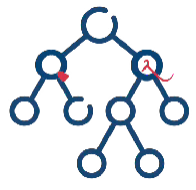
\includegraphics[height=0.9cm]{msca_logo.png}}%
  \end{center}
  \vspace{0.45cm}
  \begin{center}
    \begin{minipage}{0.1\textwidth}\centering
      \href{https://quantlet.com}{
\includegraphics[height=0.9cm]{ql_logo.png}}\end{minipage}%
    \begin{minipage}{0.78\textwidth}\centering
      {\Large\bfseries\usebeamercolor[fg]{title}\inserttitle}\par\vspace{0.25cm}
      {\large\usebeamercolor[fg]{title}\insertsubtitle}\end{minipage}%
    \begin{minipage}{0.1\textwidth}\centering
      \href{https://quantinar.com}{
\includegraphics[height=0.9cm]{qr_logo.png}}\end{minipage}
  \end{center}
  \vfill
  \hspace{0.4cm}{\bfseries\insertauthor}\par\vspace{0.12cm}
  \hspace{0.4cm}\begin{minipage}[t]{0.92\textwidth}\raggedright\footnotesize\insertinstitute\end{minipage}
  \par\vspace{0.4cm}}

% ---------------------------------------------------------------- lecture metadata
\newcommand{\nnshort}{}
\newcommand{\nnnb}{notebooks}
\newcommand{\nnrepo}{https://github.com/danpele/NEURAL_BIZ/tree/main}
% language-dependent labels (English default; \nnromanian switches to Romanian, call it before \nnlecture)
\newcommand{\txtcourse}{Neural Networks and Deep Learning}
\newcommand{\txtlecture}{Lecture}
\newcommand{\txtoutline}{Outline}
\newcommand{\txtintuition}{In one sentence:}
\newcommand{\txtjob}{In practice:}
\newcommand{\txttry}{Experiment yourself:}
\newcommand{\txtwhere}{where}
\newcommand{\txtsim}{SIMULATED DATA (teaching illustration)}
\newcommand{\txtnbsuffix}{}
\newcommand{\txtinstitute}{Bucharest University of Economic Studies (ASE), Department of Statistics and Econometrics\\
    Romanian Academy, Institute for Economic Forecasting (IPE)\\
    IDA Institute Digital Assets \textbullet\ AI4EFin \textbullet\ MSCA Digital Finance}
\newcommand{\nnromanian}{%
  \renewcommand{\txtcourse}{Rețele neuronale și deep learning}%
  \renewcommand{\txtlecture}{Cursul}%
  \renewcommand{\txtoutline}{Cuprins}%
  \renewcommand{\txtintuition}{Pe scurt:}%
  \renewcommand{\txtjob}{În practică:}%
  \renewcommand{\txttry}{Exercițiu practic:}%
  \renewcommand{\txtwhere}{unde}%
  \renewcommand{\txtsim}{DATE SIMULATE (doar pentru ilustrare)}%
  \renewcommand{\txtnbsuffix}{\string_ro}%
  \renewcommand{\txtinstitute}{Academia de Studii Economice din București (ASE), Departamentul de Statistică și Econometrie\\
    Academia Română, Institutul de Prognoză Economică (IPE)\\
    IDA Institute Digital Assets \textbullet\ AI4EFin \textbullet\ MSCA Digital Finance}}
\newcommand{\nnlecture}[2]{%
  \renewcommand{\nnshort}{\txtlecture\ #1}%
  \renewcommand{\nnnb}{notebooks/L#1\string_notebook\txtnbsuffix.ipynb}%
  \title[NN]{\txtcourse}%
  \subtitle{\txtlecture\ #1: #2}%
  \author{Prof.\ dr.\ Daniel Traian PELE}%
  \institute{\txtinstitute}%
  \date{}}

% ---------------------------------------------------------------- teaching blocks (one message per frame)
% \intuition{one plain sentence}  ->  formula with every symbol defined  ->  real-data example  ->  \manager{one line}
\newcommand{\intuition}[1]{\begin{itemize}\item {\color{MainBlue}\textbf{\txtintuition}}~#1\end{itemize}\vspace{0.6mm}}
\newcommand{\manager}[1]{\colorbox{Forest!10}{\parbox{\dimexpr\linewidth-2\fboxsep\relax}{\footnotesize
  \begin{itemize}\setlength{\itemsep}{0pt}\item \textbf{\color{Forest}\txtjob}~#1\end{itemize}}}}
% Experiment yourself: pointer to the matching notebook section
\newcommand{\tryit}[1]{{\scriptsize\href{\nnrepo/\nnnb}{%
  \raisebox{-0.15em}{
\includegraphics[height=0.85em]{ql_logo.png}}\,\textbf{\txttry}~\color{MainBlue}#1}}}
% bottom row: manager line (left) + experiment pointer (right), pinned to the bottom of the frame
\newcommand{\bottomrow}[2]{\par\vfill\noindent\begin{minipage}[b]{0.72\linewidth}#1\end{minipage}\hfill
  \begin{minipage}[b]{0.26\linewidth}\raggedleft #2\end{minipage}\par\vspace{0.5mm}}
\newcommand{\where}[1]{{\footnotesize\textbf{\txtwhere}~#1\par}}

% ---------------------------------------------------------------- helpers
% chart source line under a figure: \chartsource{Source ...; period ...}
\newcommand{\chartsource}[1]{\par\vspace{1pt}{\scriptsize\color{FooterGray}#1\par}}
% link to code: \quantlet{label}{path inside the repo}
\newcommand{\quantlet}[2]{\par\vspace{1pt}\hfill\href{\nnrepo/#2}{%
  \raisebox{-0.15em}{
\includegraphics[height=0.75em]{ql_logo.png}}\textcolor{MainBlue}{\scriptsize\ #1}}}
% inline Quantlet link for the bottom-right corner of a frame: \qlink{label}{path inside the repo}
\newcommand{\qlink}[2]{{\scriptsize\href{\nnrepo/#2}{\raisebox{-0.15em}{
\includegraphics[height=0.85em]{ql_logo.png}}\,\textcolor{MainBlue}{#1}}}}
\newcommand{\simlabel}{\colorbox{Crimson!12}{\scriptsize\bfseries\color{Crimson}\txtsim}}
\newcommand{\E}{\mathbb{E}}
\newcommand{\Var}{\operatorname{Var}}
\newcommand{\Cov}{\operatorname{Cov}}
\newcommand{\Corr}{\operatorname{Corr}}
\newcommand{\asinh}{\operatorname{asinh}}
\newcommand{\iid}{\overset{\text{i.i.d.}}{\sim}}
\newcommand{\EUR}{EUR}
% deep-learning notation (Bishop & Bishop, 2024): vectors bold lower case, matrices bold upper case
\newcommand{\R}{\mathbb{R}}
\newcommand{\vx}{\mathbf{x}}
\newcommand{\vy}{\mathbf{y}}
\newcommand{\vz}{\mathbf{z}}
\newcommand{\vh}{\mathbf{h}}
\newcommand{\vw}{\mathbf{w}}
\newcommand{\vb}{\mathbf{b}}
\newcommand{\mW}{\mathbf{W}}
\newcommand{\mX}{\mathbf{X}}
\newcommand{\btheta}{\boldsymbol{\theta}}
\newcommand{\loss}{\mathcal{L}}
\newcommand{\dataset}{\mathcal{D}}
\DeclareMathOperator*{\argmin}{arg\,min}
\DeclareMathOperator*{\argmax}{arg\,max}
\DeclareMathOperator{\softmax}{softmax}
\DeclareMathOperator{\ReLU}{ReLU}
\DeclareMathOperator{\sigm}{\sigma}

\nnlecture{12}{Large language models in finance and prompt engineering}
\begin{document}
{\setbeamertemplate{headline}{}\setbeamertemplate{footline}{}
\begin{frame}\titlepage\end{frame}}
% END-FRONT-MATTER

\begin{frame}{Learning objectives}
\small
\begin{itemize}\setlength{\itemsep}{4pt}
  \item Write the language-model objective, perplexity and the temperature of sampling, and measure them on central-bank speeches.
  \item Explain pre-training, instruction tuning and alignment from human preferences, with their loss functions.
  \item Turn a prompt into a classifier and measure zero-shot, few-shot and chain-of-thought prompts on labelled financial text, with confidence intervals.
  \item Build and evaluate retrieval-augmented generation (RAG) over real speeches, and measure hallucination.
  \item Backtest a language model used for the Value-at-Risk (VaR), and know the risks: leakage, cost, calibration.
\end{itemize}
\end{frame}

% BEGIN-ABBR

\begin{frame}{Abbreviations}
\small
\vspace{-1mm}\begin{columns}[T,onlytextwidth]
\begin{column}{0.49\textwidth}{\scriptsize\renewcommand{\arraystretch}{0.96}\begin{tabular}{@{}>{\bfseries}l@{\ \ }p{0.74\linewidth}@{}}AI & artificial intelligence\\
API & application programming interface\\
ASE & Bucharest University of Economic Studies\\
BERT & bidirectional encoder representations from transformers\\
BM25 & Best Matching 25 ranking function\\
BPE & byte-pair encoding\\
DPO & direct preference optimisation\\
ECB & European Central Bank\\
ECE & expected calibration error\\
ES & expected shortfall\\
EU & European Union\\
FinBERT & BERT model adapted to financial text\\
GARCH & generalised autoregressive conditional heteroskedasticity\\\end{tabular}}\end{column}
\begin{column}{0.49\textwidth}{\scriptsize\renewcommand{\arraystretch}{0.96}\begin{tabular}{@{}>{\bfseries}l@{\ \ }p{0.74\linewidth}@{}}GPT & generative pre-trained transformer\\
HS & historical simulation\\
IPE & Institute for Economic Forecasting, Romanian Academy\\
KL & Kullback--Leibler divergence\\
LLM & large language model\\
LoRA & low-rank adaptation\\
LR & likelihood ratio\\
MRR & mean reciprocal rank\\
RAG & retrieval-augmented generation\\
RLHF & reinforcement learning from human feedback\\
SFT & supervised fine-tuning\\
TF-IDF & term frequency--inverse document frequency\\
VaR & Value-at-Risk\\\end{tabular}}\end{column}
\end{columns}
\end{frame}

% END-ABBR


\section{Next-token prediction and large language models}

\begin{frame}{Text data in financial institutions}
\small
\begin{itemize}\setlength{\itemsep}{3pt}
  \item \textbf{Markets}
    \begin{itemize}\setlength{\itemsep}{0pt}
      \item News and social media move prices within minutes; sentiment is a signal
    \end{itemize}
  \item \textbf{Central banks}
    \begin{itemize}\setlength{\itemsep}{0pt}
      \item Speeches and minutes guide rate expectations; the European Central Bank (ECB) published 400 speeches since 2022 in our data
    \end{itemize}
  \item \textbf{Credit and risk}
    \begin{itemize}\setlength{\itemsep}{0pt}
      \item Loan files, annual reports, risk reports: reading them costs analyst hours
    \end{itemize}
  \item \textbf{This lecture}
    \begin{itemize}\setlength{\itemsep}{0pt}
      \item Open large language models (LLM) run on a laptop, measured on labelled data, never trusted on faith
    \end{itemize}
\end{itemize}
\end{frame}

\begin{frame}{A language model: next-token probabilities, trained by cross-entropy}
\footnotesize
\intuition{everything an LLM does, from answering questions to writing code, is repeated prediction of the next token.}
\begin{columns}[T,onlytextwidth]
\begin{column}{0.62\textwidth}
\[ p_{\btheta}(x_1,\dots,x_T)=\prod_{t=1}^{T}p_{\btheta}(x_t\mid x_{<t}) \]\[ \loss(\btheta)=-\frac{1}{T}\sum_{t=1}^{T}\log p_{\btheta}(x_t\mid x_{<t}),\quad \mathrm{PPL}=e^{\loss} \]{\footnotesize\begin{itemize}\setlength{\itemsep}{0pt}
  \item \textbf{\txtwhere}
    \begin{itemize}\setlength{\itemsep}{0pt}
      \item $x_t$ = token $t$
      \item $p_{\btheta}$ = softmax over the vocabulary at the last layer of a causal transformer (Lecture 7)
      \item Perplexity = the effective number of equally likely next tokens.
    \end{itemize}
\end{itemize}\par}
\end{column}
\begin{column}{0.35\textwidth}
\begin{itemize}\setlength{\itemsep}{2pt}
  \item \textbf{On ECB speeches} after July 2025, first 1,024 tokens: perplexity 14.71 (0.5B), 10.63 (1.5B), 9.43 (3B).
\end{itemize}
\end{column}
\end{columns}
\par\vfill\manager{a lower perplexity on your own documents means the model 'speaks' your domain better.}\par\vspace{0.5mm}
\par\vfill\noindent{\scriptsize\color{FooterGray}(Bishop \& Bishop, 2024, ch.\ 12)}\hfill\tryit{notebook \S1}\par\vspace{0.5mm}
\end{frame}

\begin{frame}{Subword tokens and byte-pair encoding}
\footnotesize
\intuition{frequent words are one token, rare words and numbers are split; the model never sees letters, only token indices.}
\begin{columns}[T,onlytextwidth]
\begin{column}{0.53\textwidth}
\[ (a,b)^{*}=\argmax_{(a,b)}\ \mathrm{count}(a\,b)\ \Rightarrow\ \text{merge}\ a\,b\to ab \]{\footnotesize\begin{itemize}\setlength{\itemsep}{0pt}
  \item \textbf{\txtwhere}
    \begin{itemize}\setlength{\itemsep}{0pt}
      \item Repeated until the vocabulary is full: byte-pair encoding (BPE), 151\,665 tokens in Qwen2.5
      \item WordPiece, 30\,522 tokens in a model of bidirectional encoder representations from transformers (BERT) adapted to finance (FinBERT).
    \end{itemize}
\end{itemize}\par}
\end{column}
\begin{column}{0.44\textwidth}
\begin{itemize}\setlength{\itemsep}{2pt}
  \item \textbf{Example} (20 tokens): - |  Cash |  flow |  from |  operating |  activities |  before |  investments |  was |  EUR |   | 0 | . | 8 |  - | 1 | . | 2 |  million |  ..
  \item \textbf{Financial PhraseBank}: 1.35 Qwen tokens and 1.24 WordPiece tokens per word.
\end{itemize}
\end{column}
\end{columns}
\par\vfill\manager{cost and context limits are counted in tokens, not words: budget about 1.3 tokens per English word.}\par\vspace{0.5mm}
\par\vfill\noindent{\scriptsize\color{FooterGray}(Sennrich, Haddow \& Birch, 2016)}\hfill\tryit{notebook \S1}\par\vspace{0.5mm}
\end{frame}

\begin{frame}{Sentence length in words and in tokens: two tokenisers}
\small
\intuition{the same 4\,838 sentences are a little longer in tokens than in words.}
\begin{center}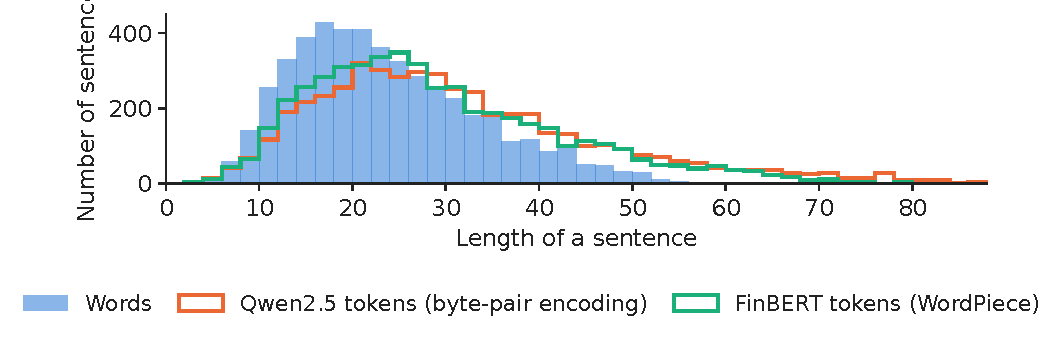
\includegraphics[width=\textwidth,height=0.550\textheight,keepaspectratio]{charts/en/tokens_per_sentence.pdf}\end{center}\vspace{-3mm}
\chartsource{Source: Financial PhraseBank (Malo et al., 2014). Data: 4,838 sentences.}
\vspace{0.5mm}
\begin{itemize}\setlength{\itemsep}{0pt}
  \item Mean: 23.1 words, 31.1 Qwen tokens, 28.6 WordPiece tokens
    \begin{itemize}\setlength{\itemsep}{0pt}
      \item An ECB speech has on average 4\,143 tokens (longest 22\,897).
    \end{itemize}
\end{itemize}
\par\vfill\noindent{\scriptsize\color{FooterGray}}\hfill\qlink{NN\_L12\_tokens\_per\_sentence}{Quantlets/L12/NN_L12_tokens_per_sentence}\par\vspace{0.5mm}
\end{frame}

\begin{frame}{Temperature reshapes the next-token distribution}
\footnotesize
\intuition{the model gives scores (logits); temperature decides how boldly we sample from them.}
\begin{columns}[T,onlytextwidth]
\begin{column}{0.5\textwidth}
\[ p_T(v\mid x_{<t})=\frac{\exp(z_v/T)}{\sum_{u}\exp(z_u/T)} \]\[ H_T=-\sum_v p_T(v)\log p_T(v) \]{\footnotesize\begin{itemize}\setlength{\itemsep}{0pt}
  \item \textbf{\txtwhere}
    \begin{itemize}\setlength{\itemsep}{0pt}
      \item $z_v$ = logit of token $v$
      \item $T\to 0$: always the most likely token (greedy)
      \item $T>1$: flatter, more diverse, more errors
      \item $H_T$ = entropy in nats.
    \end{itemize}
\end{itemize}\par}
\end{column}
\begin{column}{0.47\textwidth}
\begin{itemize}\setlength{\itemsep}{2pt}
  \item \textbf{Prompt} from the ECB speech of 30 Oct 2026: ``The inflation impact is limited: \ldots''
  \item \textbf{Top token} ``the'': 49.9\,\% at $T$ = 0.5, 10.1\,\% at 1, 0.4\,\% at 2
    \begin{itemize}\setlength{\itemsep}{0pt}
      \item Entropy 1.74, 6.20, 10.29.
    \end{itemize}
\end{itemize}
\end{column}
\end{columns}
\par\vfill\manager{for classification and extraction use temperature 0
    \begin{itemize}\setlength{\itemsep}{0pt}
      \item Reserve high temperatures for brainstorming.
    \end{itemize}}\par\vspace{0.5mm}
\par\vfill\noindent{\scriptsize\color{FooterGray}}\hfill\tryit{notebook \S2}\par\vspace{0.5mm}
\end{frame}

\begin{frame}{Next-token probabilities of a real model on a real sentence}
\small
\intuition{at low temperature almost all mass sits on one continuation; at high temperature unlikely tokens become plausible.}
\begin{center}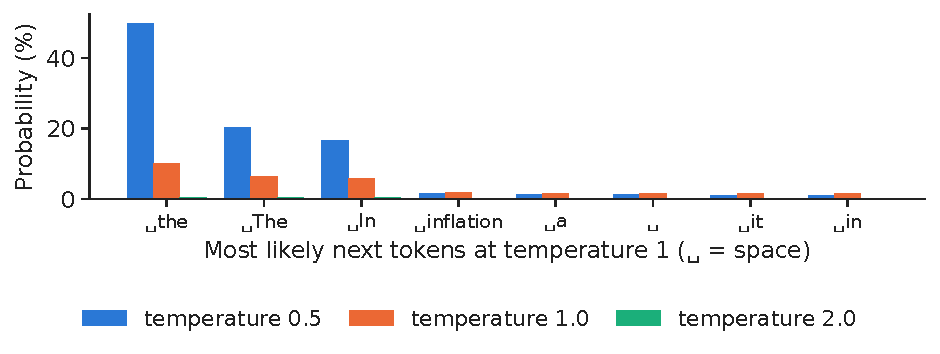
\includegraphics[width=\textwidth,height=0.585\textheight,keepaspectratio]{charts/en/next_token.pdf}\end{center}\vspace{-3mm}
\chartsource{Source: European Central Bank, speeches dataset. Data: prompt from the ECB speech of 30 Oct 2026; model Qwen2.5-1.5B-Instruct.}
\par\vfill\noindent{\scriptsize\color{FooterGray}}\hfill\qlink{NN\_L12\_next\_token}{Quantlets/L12/NN_L12_next_token}\par\vspace{0.5mm}
\end{frame}

\begin{frame}{Scaling laws: prediction loss as a power law of model size}
\footnotesize
\intuition{the loss falls as a power of the number of parameters and of training tokens.}
\begin{columns}[T,onlytextwidth]
\begin{column}{0.53\textwidth}
\[ \loss(P,D)=E+\frac{A}{P^{\alpha}}+\frac{B}{D^{\beta}} \]\[ \text{own estimate:}\ \log\loss=a+b\log P,\quad \hat b=\ensuremath{-}0.100 \]{\footnotesize\begin{itemize}\setlength{\itemsep}{0pt}
  \item \textbf{\txtwhere}
    \begin{itemize}\setlength{\itemsep}{0pt}
      \item $P$ = parameters
      \item $D$ = training tokens
      \item $E$ = irreducible loss
      \item $\alpha,\beta\approx 0.3$ (Hoffmann et al., 2022)
      \item $\hat b$ from the three Qwen2.5 sizes on ECB speeches after July 2025.
    \end{itemize}
\end{itemize}\par}
\end{column}
\begin{column}{0.44\textwidth}
\begin{itemize}\setlength{\itemsep}{2pt}
  \item \textbf{Three points are not a law}: the slope is a description of our sample, not a forecast.
  \item \textbf{Compute-optimal}: about 20 training tokens per parameter.
\end{itemize}
\end{column}
\end{columns}
\par\vfill\manager{a 3B model on a laptop costs nothing per call
    \begin{itemize}\setlength{\itemsep}{0pt}
      \item A frontier model costs per token: measure the gain first.
    \end{itemize}}\par\vspace{0.5mm}
\par\vfill\noindent{\scriptsize\color{FooterGray}(Kaplan et al., 2020; Hoffmann et al., 2022)}\hfill\tryit{notebook \S1}\par\vspace{0.5mm}
\end{frame}

\begin{frame}{Training-data cut-off and the apparent ease of older speeches}
\small
\intuition{text the model may have seen in pre-training scores a lower perplexity than text written after it.}
\begin{center}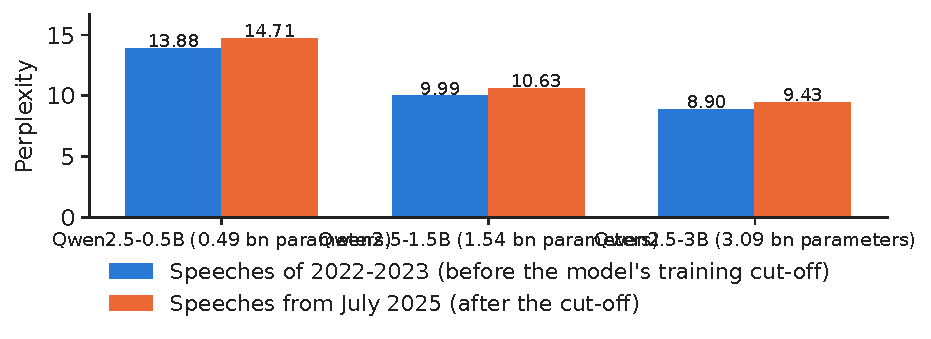
\includegraphics[width=\textwidth,height=0.309\textheight,keepaspectratio]{charts/en/perplexity_size.pdf}\end{center}\vspace{-3mm}
\chartsource{Source: European Central Bank, speeches dataset. Data: 40 + 40 speeches, first 1,024 tokens of each.}
\vspace{0.5mm}
\begin{itemize}\setlength{\itemsep}{0pt}
  \item 3B: 8.90 on 2022--2023 speeches vs 9.43 after July 2025
    \begin{itemize}\setlength{\itemsep}{0pt}
      \item Lower for the older speeches at every size.
    \end{itemize}
  \item Topics also changed
    \begin{itemize}\setlength{\itemsep}{0pt}
      \item The gap is a symptom, not a proof, of memorisation.
    \end{itemize}
\end{itemize}
\par\vfill\manager{evaluate an LLM on documents written after its training cut-off, or the score may be inflated by leakage.}\par\vspace{0.5mm}
\par\vfill\noindent{\scriptsize\color{FooterGray}}\hfill\qlink{NN\_L12\_perplexity\_size}{Quantlets/L12/NN_L12_perplexity_size}\par\vspace{0.5mm}
\end{frame}


\section{Pre-training, instruction tuning and alignment}

\begin{frame}{Three training stages of a language-model assistant}
\small
\begin{center}\begin{tikzpicture}\node[draw, rounded corners, fill=MainBlue!12, text width=2.55cm, align=center, minimum height=1.05cm, font=\scriptsize] (n0) at (0.0,0) {\textbf{Pre-training}\\trillions of tokens\\next-token loss};\node[draw, rounded corners, fill=Ser2!12, text width=2.55cm, align=center, minimum height=1.05cm, font=\scriptsize] (n1) at (3.05,0) {\textbf{Supervised fine-tuning}\\(prompt, answer) pairs};\node[draw, rounded corners, fill=Ser3!12, text width=2.55cm, align=center, minimum height=1.05cm, font=\scriptsize] (n2) at (6.1,0) {\textbf{Preferences}\\answer A better than B};\node[draw, rounded corners, fill=Ser7!12, text width=2.55cm, align=center, minimum height=1.05cm, font=\scriptsize] (n3) at (9.149999999999999,0) {\textbf{Assistant}\\follows instructions};\draw[-{Stealth}, thick] (n0.east) -- (n1.west);\draw[-{Stealth}, thick] (n1.east) -- (n2.west);\draw[-{Stealth}, thick] (n2.east) -- (n3.west);\end{tikzpicture}\end{center}\begin{itemize}\setlength{\itemsep}{3pt}
  \item \textbf{Generative pre-trained transformer (GPT)}: stage 1 alone gives a model that continues text, not one that answers.
  \item \textbf{Supervised fine-tuning (SFT)} teaches the format
    \begin{itemize}\setlength{\itemsep}{0pt}
      \item \textbf{reinforcement learning from human feedback (RLHF)} or \textbf{direct preference optimisation (DPO)} teaches which answers people prefer.
    \end{itemize}
  \item \textbf{Qwen2.5-Instruct} (Qwen Team, 2024): 18 trillion pre-training tokens, then SFT and preference optimisation.
\end{itemize}
\par\vfill\noindent{\scriptsize\color{FooterGray}(Ouyang et al., 2022; Qwen Team, 2024)}\par\vspace{0.5mm}
\end{frame}

\begin{frame}{Instruction tuning is next-token loss on the answer only}
\footnotesize
\intuition{the model sees prompt and answer, but is graded only on the answer tokens.}
\begin{columns}[T,onlytextwidth]
\begin{column}{0.53\textwidth}
\[ \loss_{\text{SFT}}(\btheta)=-\sum_{(\mathbf x,\mathbf y)\in\dataset}\ \sum_{t=1}^{|\mathbf y|}\log p_{\btheta}\big(y_t\mid \mathbf x,\mathbf y_{<t}\big) \]{\footnotesize\begin{itemize}\setlength{\itemsep}{0pt}
  \item \textbf{\txtwhere}
    \begin{itemize}\setlength{\itemsep}{0pt}
      \item $\mathbf x$ = instruction (with a chat template: system, user, assistant roles)
      \item $\mathbf y$ = reference answer
      \item $\dataset$ = tens of thousands to millions of pairs.
    \end{itemize}
\end{itemize}\par}
\end{column}
\begin{column}{0.44\textwidth}
\begin{itemize}\setlength{\itemsep}{2pt}
  \item \textbf{Low-rank adaptation (LoRA)}: train $\mathbf W=\mathbf W_0+\mathbf B\mathbf A$ with $\mathbf B\in\R^{d\times r}$, $\mathbf A\in\R^{r\times k}$, $r\ll d$
    \begin{itemize}\setlength{\itemsep}{0pt}
      \item $\mathbf W_0$ frozen.
    \end{itemize}
  \item \textbf{A $4096\times4096$ layer, $r=8$}: 65,536 trainable weights instead of 16.8 million.
\end{itemize}
\end{column}
\end{columns}
\par\vfill\manager{a bank adapts an open model to its own documents with LoRA on one graphics card, keeping data in-house.}\par\vspace{0.5mm}
\par\vfill\noindent{\scriptsize\color{FooterGray}(Hu et al., 2022)}\par\vspace{0.5mm}
\end{frame}

\begin{frame}{Alignment: reward models and direct preference optimisation}
\footnotesize
\intuition{people say which of two answers is better; the model is pushed towards preferred answers without drifting too far.}
\begin{columns}[T,onlytextwidth]
\begin{column}{0.56\textwidth}
\[ \Pr(y_w\succ y_l\mid x)=\sigma\big(r_\phi(x,y_w)-r_\phi(x,y_l)\big) \]\[ \max_{\btheta}\ \E\big[r_\phi(x,y)\big]-\beta\,\mathrm{KL}\big(p_{\btheta}\,\|\,p_{\text{SFT}}\big) \]\[ \loss_{\text{DPO}}=-\log\sigma\Big(\beta\log\tfrac{p_{\btheta}(y_w|x)}{p_{\text{SFT}}(y_w|x)}-\beta\log\tfrac{p_{\btheta}(y_l|x)}{p_{\text{SFT}}(y_l|x)}\Big) \]{\footnotesize\begin{itemize}\setlength{\itemsep}{0pt}
  \item \textbf{\txtwhere}
    \begin{itemize}\setlength{\itemsep}{0pt}
      \item $y_w,y_l$ = preferred and rejected answers
      \item $r_\phi$ = reward model (Bradley--Terry)
      \item $\sigma$ = logistic function
      \item Kullback--Leibler (KL) penalty with weight $\beta$ keeps the model close to the SFT model.
    \end{itemize}
\end{itemize}\par}
\end{column}
\begin{column}{0.41\textwidth}
\begin{itemize}\setlength{\itemsep}{2pt}
  \item \textbf{RLHF} fits $r_\phi$, then optimises the policy
    \begin{itemize}\setlength{\itemsep}{0pt}
      \item \textbf{DPO} skips the reward model.
    \end{itemize}
  \item \textbf{Side effect}: aligned models sound confident
    \begin{itemize}\setlength{\itemsep}{0pt}
      \item Confidence is not accuracy (calibration, below).
    \end{itemize}
\end{itemize}
\end{column}
\end{columns}
\par\vfill\manager{alignment sets tone and safety, not financial knowledge: evaluate on your task.}\par\vspace{0.5mm}
\par\vfill\noindent{\scriptsize\color{FooterGray}(Ouyang et al., 2022; Rafailov et al., 2023)}\par\vspace{0.5mm}
\end{frame}

\begin{frame}{The open models used in this lecture}
\small
{\footnotesize\renewcommand{\arraystretch}{1.05}\setlength{\tabcolsep}{4pt}
\begin{tabular}{@{}p{0.33\textwidth}rp{0.45\textwidth}@{}}\toprule
Model & Parameters & Role here \\ \midrule
Qwen2.5-0.5B-Instruct & 0.49 bn & perplexity, zero-shot classification \\
Qwen2.5-1.5B-Instruct & 1.54 bn & next-token probabilities, few-shot, embeddings \\
Qwen2.5-3B-Instruct & 3.09 bn & best prompts, chain-of-thought, question answering, LLM-VaR \\
BAAI bge-small-en-v1.5 & 33 m & dense retrieval embeddings (384 dimensions) \\
Term frequency--inverse document frequency (TF-IDF) + logistic regression & -- & classical benchmark trained on the labelled data \\
\bottomrule\end{tabular}}
\par\vspace{0.5mm}{\scriptsize \begin{itemize}\setlength{\itemsep}{0pt}
  \item All models run locally on a laptop; no text leaves the machine and no application programming interface (API) is paid.
  \item TF-IDF: word and word-pair counts weighted by their rarity across documents.
\end{itemize}}
\par\vfill\noindent{\scriptsize\color{FooterGray}(Qwen Team, 2024; Xiao et al., 2023)}\par\vspace{0.5mm}
\end{frame}


\section{Evaluation of prompt engineering on labelled data}

\begin{frame}{Structure of a prompt}
\small
\begin{columns}[T,onlytextwidth]
\begin{column}{0.5\textwidth}
\begin{itemize}\setlength{\itemsep}{3pt}
  \item \textbf{System}
    \begin{itemize}\setlength{\itemsep}{0pt}
      \item Role and rules: ``You are a careful financial analyst.''
    \end{itemize}
  \item \textbf{Instruction}
    \begin{itemize}\setlength{\itemsep}{0pt}
      \item Task, label set, output format: ``Answer with one word: positive, negative or neutral.''
    \end{itemize}
  \item \textbf{Examples} (optional)
    \begin{itemize}\setlength{\itemsep}{0pt}
      \item $k$ labelled input--answer pairs: few-shot
    \end{itemize}
  \item \textbf{Input}
    \begin{itemize}\setlength{\itemsep}{0pt}
      \item The sentence, tweet or document to process
    \end{itemize}
\end{itemize}
\end{column}
\begin{column}{0.47\textwidth}
\begin{itemize}\setlength{\itemsep}{3pt}
  \item \textbf{Variants we test}
    \begin{itemize}\setlength{\itemsep}{0pt}
      \item Zero-shot: instruction + input
      \item Few-shot: 3 to 24 examples
      \item Chain-of-thought: ``explain, then answer''
      \item Five paraphrases of the instruction
    \end{itemize}
  \item \textbf{Rule of this lecture}
    \begin{itemize}\setlength{\itemsep}{0pt}
      \item Every prompt is a model: it is scored on a held-out test set
    \end{itemize}
\end{itemize}
\end{column}
\end{columns}
\par\vfill\noindent{\scriptsize\color{FooterGray}(Brown et al., 2020; Wei et al., 2022)}\par\vspace{0.5mm}
\end{frame}

\begin{frame}{A prompt as a classifier: probabilities of the label words}
\footnotesize
\intuition{read the probability of each label at the answer position: no text generation, no parsing, and a calibrated-looking score.}
\begin{columns}[T,onlytextwidth]
\begin{column}{0.53\textwidth}
\[ \hat p(c\mid x)=\frac{\sum_{v\in\mathcal V_c}p_{\btheta}(v\mid \mathrm{prompt}(x))}{\sum_{c'}\sum_{v\in\mathcal V_{c'}}p_{\btheta}(v\mid \mathrm{prompt}(x))} \]\[ \hat c=\argmax_c\hat p(c\mid x) \]{\footnotesize\begin{itemize}\setlength{\itemsep}{0pt}
  \item \textbf{\txtwhere}
    \begin{itemize}\setlength{\itemsep}{0pt}
      \item $\mathcal V_c$ = first tokens of the label word $c$ in its spellings (``positive'', `` Positive'', \ldots)
      \item The prompt ends where the assistant's answer starts.
    \end{itemize}
\end{itemize}\par}
\end{column}
\begin{column}{0.44\textwidth}
\begin{itemize}\setlength{\itemsep}{2pt}
  \item \textbf{Fast}: one forward pass per item
    \begin{itemize}\setlength{\itemsep}{0pt}
      \item The shared instruction and examples are encoded once (key--value cache).
    \end{itemize}
  \item \textbf{Comparable}: the same macro-F1 and confidence intervals as any classifier.
\end{itemize}
\end{column}
\end{columns}
\par\vfill\manager{constrain the output space
    \begin{itemize}\setlength{\itemsep}{0pt}
      \item Free text answers need parsing and fail silently.
    \end{itemize}}\par\vspace{0.5mm}
\par\vfill\noindent{\scriptsize\color{FooterGray}(Zhao et al., 2021)}\hfill\tryit{notebook \S3}\par\vspace{0.5mm}
\end{frame}

\begin{frame}{Two labelled data sets: financial news and finance tweets}
\small
{\footnotesize\renewcommand{\arraystretch}{1.05}\setlength{\tabcolsep}{4pt}
\begin{tabular}{@{}p{0.27\textwidth}p{0.3\textwidth}rrp{0.17\textwidth}@{}}\toprule
Data set & Labels & Train & Test & Neutral share (test) \\ \midrule
Financial PhraseBank, 100\,\% agreement & positive, negative, neutral & 1581 & 678 & 61.4\,\% \\
Twitter financial news & bullish, bearish, neutral & 9\,543 & 900 & 65.6\,\% \\
\bottomrule\end{tabular}}
\par\vspace{0.5mm}{\scriptsize \begin{itemize}\setlength{\itemsep}{0pt}
  \item PhraseBank: 4\,838 sentences from news about Finnish listed companies, labelled by 5--8 annotators; we use the 2\,259 with unanimous labels, split 70/30 stratified (seed 20261108).
  \item Twitter: published split; test = stratified sample of 900 of the 2\,388 validation tweets.
  \item The examples for few-shot prompts are drawn from the training part only.
\end{itemize}}
\par\vfill\noindent{\scriptsize\color{FooterGray}(Malo et al., 2014)}\par\vspace{0.5mm}
\end{frame}

\begin{frame}{Prompted LLMs against a trained benchmark}
\small
\intuition{no single strategy wins everywhere; the trained classifiers use the labelled data, the prompts do not.}
\begin{center}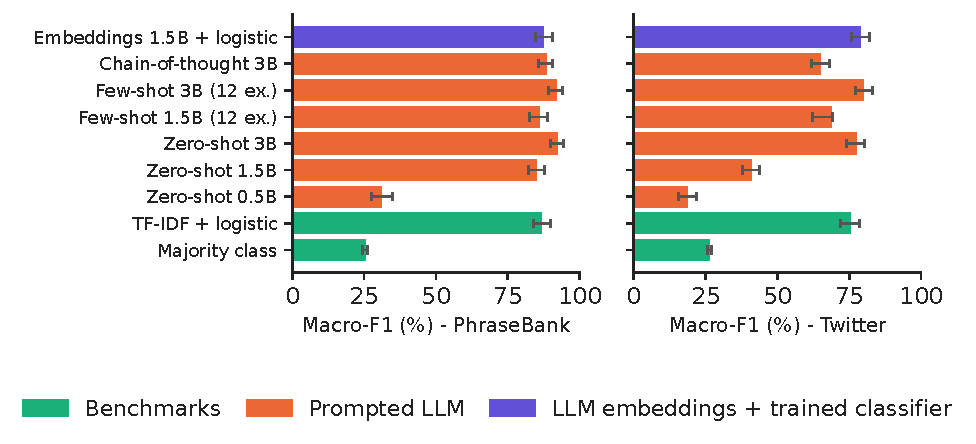
\includegraphics[width=\textwidth,height=0.442\textheight,keepaspectratio]{charts/en/prompt_results.pdf}\end{center}\vspace{-3mm}
\chartsource{Source: Financial PhraseBank (Malo et al., 2014) and Twitter financial news (zeroshot). Data: test sets: 678 sentences (100\,\% agreement) and 900 tweets; 95\,\% bootstrap intervals.}
\vspace{0.5mm}
\begin{itemize}\setlength{\itemsep}{0pt}
  \item Best on PhraseBank: zero-shot 3B (92.2\,\%)
    \begin{itemize}\setlength{\itemsep}{0pt}
      \item On Twitter: few-shot 3B (79.8\,\%)
      \item Zero-shot 3B: 92.2\,\% and 77.4\,\%.
    \end{itemize}
\end{itemize}
\par\vfill\noindent{\scriptsize\color{FooterGray}}\hfill\qlink{NN\_L12\_prompt\_results}{Quantlets/L12/NN_L12_prompt_results}\par\vspace{0.5mm}
\end{frame}

\begin{frame}{Accuracy and macro-F1 with 95\,\% bootstrap intervals}
\small
{\scriptsize\renewcommand{\arraystretch}{1.05}\setlength{\tabcolsep}{4pt}
\begin{tabular}{@{}lrrlrrl@{}}\toprule
Method & Acc. & F1 & 95\,\% int. & Acc. & F1 & 95\,\% int. \\ \midrule
 & \multicolumn{3}{c}{PhraseBank} & \multicolumn{3}{c}{Twitter} \\
majority class & 61.4 & \cellcolor{Crimson!55}25.4 & [24.4; 26.3] & 65.6 & \cellcolor{Crimson!55}26.4 & [25.7; 27.1] \\
TF-IDF + logistic & 90.3 & \cellcolor{Forest!46}86.9 & [83.8; 90.0] & 81.4 & \cellcolor{Forest!46}75.5 & [71.9; 78.7] \\
zero-shot 0.5B & 62.8 & \cellcolor{Crimson!53}31.0 & [27.5; 34.8] & 23.1 & \cellcolor{Crimson!55}18.7 & [15.7; 21.9] \\
zero-shot 1.5B & 85.3 & \cellcolor{Forest!42}85.1 & [82.2; 87.9] & 37.8 & \cellcolor{Crimson!31}40.9 & [37.9; 43.7] \\
zero-shot 3B & 93.1 & \cellcolor{Forest!55}92.2 & [89.8; 94.4] & 81.2 & \cellcolor{Forest!50}77.4 & [74.2; 80.3] \\
few-shot 1.5B & 87.8 & \cellcolor{Forest!44}85.9 & [82.5; 88.7] & 73.7 & \cellcolor{Forest!31}68.8 & [62.3; 69.1] \\
few-shot 3B & 93.4 & \cellcolor{Forest!55}92.1 & [89.2; 94.1] & 84.3 & \cellcolor{Forest!55}79.8 & [77.2; 83.2] \\
chain-of-thought 3B & 88.5 & \cellcolor{Forest!48}88.4 & [85.7; 90.7] & 64.7 & \cellcolor{Forest!23}65.1 & [62.0; 68.0] \\
embeddings 1.5B + logistic & 91.3 & \cellcolor{Forest!47}87.5 & [84.5; 90.7] & 83.0 & \cellcolor{Forest!53}79.0 & [75.7; 82.0] \\
\bottomrule\end{tabular}}
\par\vspace{0.5mm}{\scriptsize \begin{itemize}\setlength{\itemsep}{0pt}
  \item Macro-F1 = mean of the three per-class F1 scores, so the small negative class counts as much as neutral; intervals from 1,000 bootstrap resamples of the test set; few-shot = mean of 3 seeds.
  \item Int. = 95\,\% bootstrap interval of the macro-F1.
\end{itemize}}
\par\vfill\noindent{\scriptsize\color{FooterGray}(own computation)}\hfill\tryit{notebook \S3}\par\vspace{0.5mm}
\end{frame}

\begin{frame}{Effect of the number of examples in the prompt}
\small
\intuition{in-context learning: the examples change the output without changing a single weight.}
\vspace{-1mm}\[ \hat c=\argmax_c\,p_{\btheta}\big(c\mid (x_1,c_1),\dots,(x_k,c_k),x\big) \]\vspace{-2mm}
\begin{center}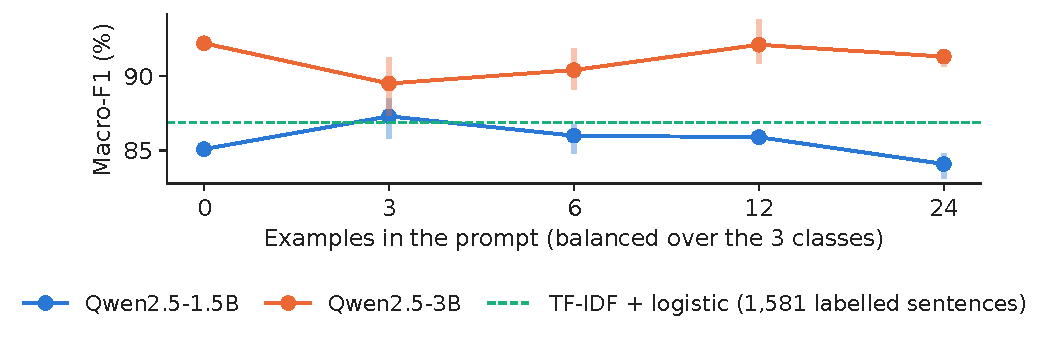
\includegraphics[width=\textwidth,height=0.456\textheight,keepaspectratio]{charts/en/fewshot_curve.pdf}\end{center}\vspace{-3mm}
\chartsource{Source: Financial PhraseBank (Malo et al., 2014). Data: test set of 678 sentences; bars = range over 3 seeds.}
\vspace{0.5mm}
\begin{itemize}\setlength{\itemsep}{0pt}
  \item 1.5B: 85.1\,\% with no example, 84.1\,\% with 24
    \begin{itemize}\setlength{\itemsep}{0pt}
      \item 3B: 92.2\,\% and 91.3\,\%
      \item Seeds move 3B with 12 examples between 91.0 and 93.6\,\%.
    \end{itemize}
\end{itemize}
\par\vfill\noindent{\scriptsize\color{FooterGray}}\hfill\qlink{NN\_L12\_fewshot\_curve}{Quantlets/L12/NN_L12_fewshot_curve}\par\vspace{0.5mm}
\end{frame}

\begin{frame}{Prompt sensitivity: effect of rewording the instruction}
\small
\intuition{five instructions with the same meaning, the same model and data: the spread is a source of model risk.}
\begin{center}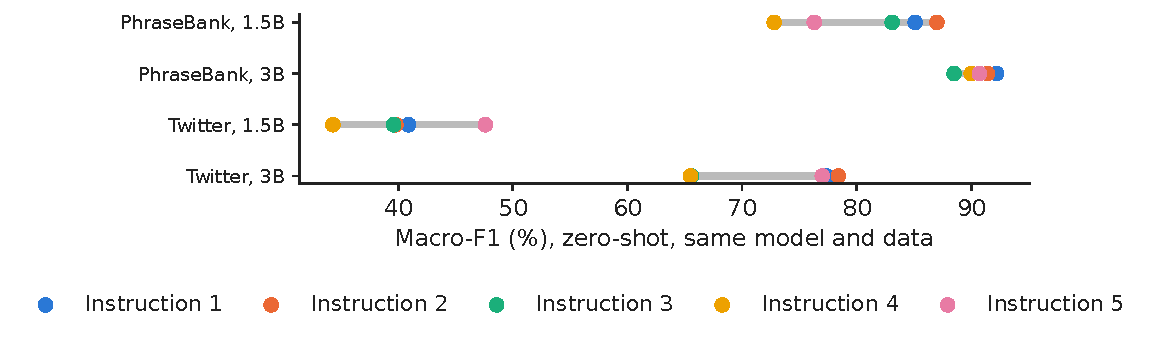
\includegraphics[width=\textwidth,height=0.364\textheight,keepaspectratio]{charts/en/prompt_sensitivity.pdf}\end{center}\vspace{-3mm}
\chartsource{Source: Financial PhraseBank and Twitter financial news. Data: test sets as above; five paraphrases of the instruction.}
\vspace{0.5mm}
\begin{itemize}\setlength{\itemsep}{0pt}
  \item Range of macro-F1 over the five wordings: PhraseBank 3B 3.6 points, Twitter 3B 12.9 points, Twitter 1.5B 13.3 points.
\end{itemize}
\par\vfill\manager{choose the prompt on a validation set and freeze it, like any hyper-parameter
    \begin{itemize}\setlength{\itemsep}{0pt}
      \item Never on the test set.
    \end{itemize}}\par\vspace{0.5mm}
\par\vfill\noindent{\scriptsize\color{FooterGray}}\hfill\qlink{NN\_L12\_prompt\_sensitivity}{Quantlets/L12/NN_L12_prompt_sensitivity}\par\vspace{0.5mm}
\end{frame}

\begin{frame}{Chain-of-thought: written reasoning before the answer}
\footnotesize
\intuition{generated reasoning tokens become extra context for the final label.}
\begin{columns}[T,onlytextwidth]
\begin{column}{0.53\textwidth}
\[ p(c\mid x)=\sum_{r}p(r\mid x)\,p(c\mid x,r)\ \approx\ p(c\mid x,\hat r) \]{\footnotesize\begin{itemize}\setlength{\itemsep}{0pt}
  \item \textbf{\txtwhere}
    \begin{itemize}\setlength{\itemsep}{0pt}
      \item $r$ = reasoning text, $\hat r$ = the greedy one (at most two sentences, on average 35.9 words)
      \item The label is parsed from ``Label: \ldots''
      \item Parsed for 100.0\,\% of PhraseBank answers.
    \end{itemize}
\end{itemize}\par}
\end{column}
\begin{column}{0.44\textwidth}
\begin{itemize}\setlength{\itemsep}{2pt}
  \item \textbf{Macro-F1}: PhraseBank 88.4\,\% (zero-shot 3B 92.2\,\%)
    \begin{itemize}\setlength{\itemsep}{0pt}
      \item Twitter 65.1\,\% (77.4\,\%).
    \end{itemize}
  \item \textbf{Cost}: 389 ms per sentence against 48.5 ms for zero-shot.
\end{itemize}
\end{column}
\end{columns}
\par\vfill\manager{chain-of-thought helps on multi-step reasoning
    \begin{itemize}\setlength{\itemsep}{0pt}
      \item For one-word labels on short text, test before paying for it.
    \end{itemize}}\par\vspace{0.5mm}
\par\vfill\noindent{\scriptsize\color{FooterGray}(Wei et al., 2022)}\hfill\tryit{notebook \S5}\par\vspace{0.5mm}
\end{frame}

\begin{frame}{An example of a chain-of-thought answer}
\small
\begin{itemize}\setlength{\itemsep}{4pt}
  \item \textbf{Input} (PhraseBank test set)
    \begin{itemize}\setlength{\itemsep}{0pt}
      \item ``CapMan said the deal 's effect on its cash flow for 2009 totals EUR3 .4 m , but the transaction would not affect its financial results for 2009 as it was executed at fair value .''
    \end{itemize}
  \item \textbf{Output} of Qwen2.5-3B-Instruct, temperature 0
    \begin{itemize}\setlength{\itemsep}{0pt}
      \item ``Reasoning: The sentence indicates that the deal has a positive impact on CapMan's cash flow, which is generally seen as beneficial for investors. However, it also clarifies that the transaction does not affect their financial results, suggesting no immediate change to profitability. Given these points, the overall sentiment leans positive as it highlights a direct benefit. Label: positive''
    \end{itemize}
  \item \textbf{How to read it}
    \begin{itemize}\setlength{\itemsep}{0pt}
      \item The reasoning is a plausible story, not a faithful trace of the computation
      \item Audit the label against the data, not the explanation against your intuition
    \end{itemize}
\end{itemize}
\par\vfill\noindent{\scriptsize\color{FooterGray}(own computation)}\par\vspace{0.5mm}
\end{frame}

\begin{frame}{Calibration of the label probabilities on real data}
\small
\intuition{a probability of 0.9 should be right nine times in ten; points below the diagonal mean over-confidence.}
\vspace{-1mm}\[ \mathrm{ECE}=\sum_{b=1}^{B}\frac{|S_b|}{n}\,\big|\mathrm{acc}(S_b)-\mathrm{conf}(S_b)\big| \]\vspace{-2mm}
\begin{center}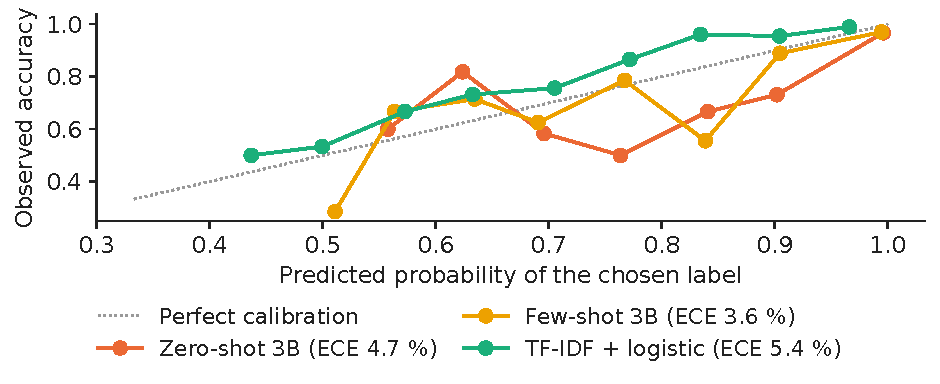
\includegraphics[width=\textwidth,height=0.345\textheight,keepaspectratio]{charts/en/calibration.pdf}\end{center}\vspace{-3mm}
\chartsource{Source: Financial PhraseBank (Malo et al., 2014). Data: test set of 678 sentences, 10 bins.}
\vspace{0.5mm}
\begin{itemize}\setlength{\itemsep}{0pt}
  \item Expected calibration error (ECE): zero-shot 3B 4.7\,\%, few-shot 3B 3.6\,\%, TF-IDF + logistic 5.4\,\%.
\end{itemize}
\par\vfill\manager{recalibrate on a validation set (temperature scaling) before using LLM probabilities as risk scores.}\par\vspace{0.5mm}
\par\vfill\noindent{\scriptsize\color{FooterGray}(Guo et al., 2017)}\hfill\qlink{NN\_L12\_calibration}{Quantlets/L12/NN_L12_calibration}\par\vspace{0.5mm}
\end{frame}

\begin{frame}{Accuracy by level of annotator agreement}
\small
\intuition{sentences that split the annotators are genuinely ambiguous; no model reaches the unanimous-case accuracy on them.}
\begin{center}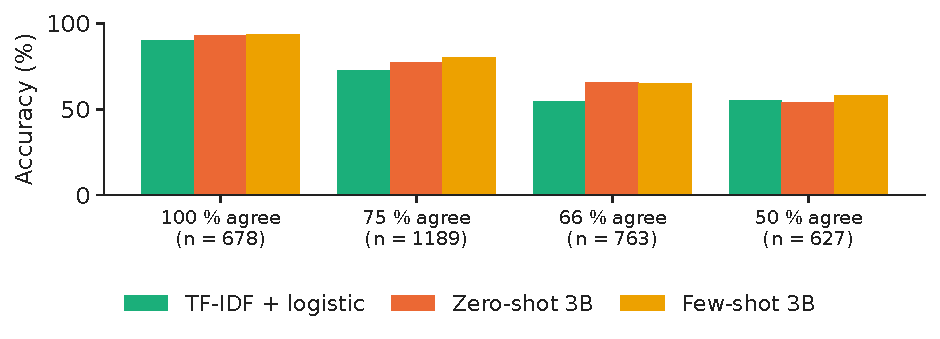
\includegraphics[width=\textwidth,height=0.377\textheight,keepaspectratio]{charts/en/agreement.pdf}\end{center}\vspace{-3mm}
\chartsource{Source: Financial PhraseBank (Malo et al., 2014). Data: sentences never used for training or for examples.}
\vspace{0.5mm}
\begin{itemize}\setlength{\itemsep}{0pt}
  \item Zero-shot 3B: 93.1\,\% at 100\,\% agreement, 53.7\,\% at 50\,\%
    \begin{itemize}\setlength{\itemsep}{0pt}
      \item TF-IDF: 90.3\,\% and 54.9\,\%.
    \end{itemize}
\end{itemize}
\par\vfill\manager{report the label quality of your test set
    \begin{itemize}\setlength{\itemsep}{0pt}
      \item A model cannot be more certain than the people who labelled it.
    \end{itemize}}\par\vspace{0.5mm}
\par\vfill\noindent{\scriptsize\color{FooterGray}}\hfill\qlink{NN\_L12\_agreement}{Quantlets/L12/NN_L12_agreement}\par\vspace{0.5mm}
\end{frame}

\begin{frame}{Confusion matrix of the best prompt}
\small
\begin{columns}[T,onlytextwidth]
\begin{column}{0.5\textwidth}
{\footnotesize\renewcommand{\arraystretch}{1.05}\setlength{\tabcolsep}{4pt}
\begin{tabular}{@{}lrrr@{}}\toprule
True \textbackslash{} predicted & positive & negative & neutral \\ \midrule
positive & \cellcolor{MainBlue!24}156 & 2 & \cellcolor{MainBlue!2}13 \\
negative & 1 & \cellcolor{MainBlue!13}82 & \cellcolor{MainBlue!1}8 \\
neutral & \cellcolor{MainBlue!3}20 & 3 & \cellcolor{MainBlue!60}\textcolor{white}{393} \\
\bottomrule\end{tabular}}
\end{column}
\begin{column}{0.47\textwidth}
\begin{itemize}\setlength{\itemsep}{4pt}
  \item \textbf{Model}: zero-shot 3B, PhraseBank test set.
  \item \textbf{Neutral read as positive}: 20 sentences
    \begin{itemize}\setlength{\itemsep}{0pt}
      \item \textbf{positive read as neutral}: 13.
    \end{itemize}
  \item \textbf{Negative and positive} are rarely swapped: 1 + 2.
\end{itemize}
\end{column}
\end{columns}
\par\vspace{0.5mm}{\scriptsize \begin{itemize}\setlength{\itemsep}{0pt}
  \item Errors sit on the neutral border: ``profit rose but less than expected'' is the hard case, not good versus bad news.
\end{itemize}}
\par\vfill\noindent{\scriptsize\color{FooterGray}(own computation)}\hfill\tryit{notebook \S6}\par\vspace{0.5mm}
\end{frame}

\begin{frame}{Cost against accuracy: milliseconds per sentence on a laptop}
\small
\intuition{the cheapest model is thousands of times faster than the slowest; the accuracy gap is small.}
\begin{center}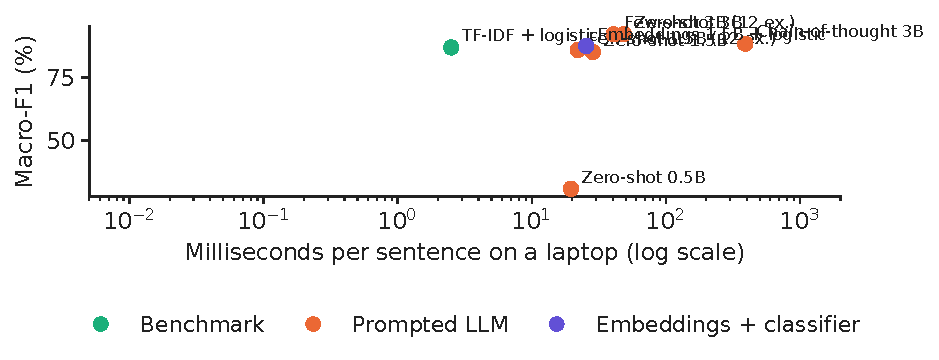
\includegraphics[width=\textwidth,height=0.300\textheight,keepaspectratio]{charts/en/cost_accuracy.pdf}\end{center}\vspace{-3mm}
\chartsource{Source: Financial PhraseBank (Malo et al., 2014). Data: test set of 678 sentences; time measured on a laptop graphics processor.}
\vspace{0.5mm}
\begin{itemize}\setlength{\itemsep}{0pt}
  \item TF-IDF: 2.50 ms per sentence
    \begin{itemize}\setlength{\itemsep}{0pt}
      \item Zero-shot 3B: 48.5 ms
      \item Chain-of-thought 3B: 389 ms.
    \end{itemize}
\end{itemize}
\par\vfill\manager{with labels, train a small model
    \begin{itemize}\setlength{\itemsep}{0pt}
      \item Without labels, prompt an LLM
      \item For millions of documents, the cost decides.
    \end{itemize}}\par\vspace{0.5mm}
\par\vfill\noindent{\scriptsize\color{FooterGray}}\hfill\qlink{NN\_L12\_cost\_accuracy}{Quantlets/L12/NN_L12_cost_accuracy}\par\vspace{0.5mm}
\end{frame}

\begin{frame}{LLM embeddings with a small classifier as a low-cost alternative to fine-tuning}
\footnotesize
\intuition{freeze the language model, average its last hidden states, and fit a logistic regression on top.}
\begin{columns}[T,onlytextwidth]
\begin{column}{0.53\textwidth}
\[ \mathbf e(x)=\frac{1}{|x|}\sum_{t=1}^{|x|}\mathbf h^{(L)}_t,\qquad \hat p(c\mid x)=\softmax\big(\mathbf W\mathbf e(x)+\mathbf b\big)_c \]{\footnotesize\begin{itemize}\setlength{\itemsep}{0pt}
  \item \textbf{\txtwhere}
    \begin{itemize}\setlength{\itemsep}{0pt}
      \item $\mathbf h^{(L)}_t\in\R^{1536}$ = last hidden state of Qwen2.5-1.5B
      \item $\mathbf W$ fitted with an L2 penalty chosen by 5-fold cross-validation.
    \end{itemize}
\end{itemize}\par}
\end{column}
\begin{column}{0.44\textwidth}
\begin{itemize}\setlength{\itemsep}{2pt}
  \item \textbf{Macro-F1}: PhraseBank 87.5\,\%, Twitter 79.0\,\%.
  \item \textbf{Uses the labels} like TF-IDF, but with the language knowledge of the LLM.
\end{itemize}
\end{column}
\end{columns}
\par\vfill\manager{before full fine-tuning, try a probe: minutes on a laptop, no gradient through the LLM.}\par\vspace{0.5mm}
\par\vfill\noindent{\scriptsize\color{FooterGray}}\hfill\tryit{notebook \S6}\par\vspace{0.5mm}
\end{frame}


\section{Retrieval-augmented generation on ECB speeches}

\begin{frame}{RAG: document retrieval followed by answer generation}
\small
\begin{center}\begin{tikzpicture}\node[draw, rounded corners, fill=MainBlue!12, text width=2.55cm, align=center, minimum height=1.05cm, font=\scriptsize] (n0) at (0.0,0) {\textbf{Question}};\node[draw, rounded corners, fill=Ser3!12, text width=2.55cm, align=center, minimum height=1.05cm, font=\scriptsize] (n1) at (3.05,0) {\textbf{Retriever}\\BM25 + dense\\top-$k$ chunks};\node[draw, rounded corners, fill=Ser2!12, text width=2.55cm, align=center, minimum height=1.05cm, font=\scriptsize] (n2) at (6.1,0) {\textbf{Prompt}\\documents + question};\node[draw, rounded corners, fill=Ser7!12, text width=2.55cm, align=center, minimum height=1.05cm, font=\scriptsize] (n3) at (9.149999999999999,0) {\textbf{LLM answer}\\with sources};\draw[-{Stealth}, thick] (n0.east) -- (n1.west);\draw[-{Stealth}, thick] (n1.east) -- (n2.west);\draw[-{Stealth}, thick] (n2.east) -- (n3.west);\end{tikzpicture}\end{center}\vspace{-2mm}\[ p(y\mid q)\approx\sum_{z\in\mathrm{top}_k(q)}p_\eta(z\mid q)\,p_{\btheta}(y\mid q,z) \]\begin{itemize}\setlength{\itemsep}{2pt}
  \item \textbf{Retrieval-augmented generation (RAG)}: $z$ = retrieved chunk, $p_\eta$ = retriever, $p_{\btheta}$ = generator.
  \item \textbf{Our corpus}: 400 ECB speeches, 8\,400 chunks of 200 words (overlap 50).
\end{itemize}
\par\vfill\noindent{\scriptsize\color{FooterGray}(Lewis et al., 2020)}\par\vspace{0.5mm}
\end{frame}

\begin{frame}{Three retrievers: shared words, weighted terms, dense embeddings}
\footnotesize
\intuition{lexical retrievers match words, dense ones match meaning, a hybrid combines both; the query here is a speech title.}
\begin{columns}[T,onlytextwidth]
\begin{column}{0.64\textwidth}
\[ \mathrm{BM25}(q,z)=\sum_{w\in q}\mathrm{idf}(w)\frac{f(w,z)(k_1+1)}{f(w,z)+k_1\big(1-b+b\frac{|z|}{\overline{|z|}}\big)} \]\[ s_{\text{dense}}=\cos\big(\mathbf e(q),\mathbf e(z)\big),\quad s_{\text{RRF}}(z)=\sum_{m}\frac{1}{60+\mathrm{rank}_m(z)} \]{\footnotesize\begin{itemize}\setlength{\itemsep}{0pt}
  \item \textbf{\txtwhere}
    \begin{itemize}\setlength{\itemsep}{0pt}
      \item $f(w,z)$ = count of word $w$ in chunk $z$
      \item $k_1=1.5$, $b=0.75$
      \item Best Matching 25 (BM25)
      \item $\mathbf e$ = bge-small embedding
      \item RRF = rank fusion.
    \end{itemize}
\end{itemize}\par}
\end{column}
\begin{column}{0.33\textwidth}
\begin{itemize}\setlength{\itemsep}{2pt}
  \item \textbf{Mean reciprocal rank (MRR)}: BM25 0.515, dense 0.567, hybrid 0.622.
\end{itemize}
\end{column}
\end{columns}
\par\vfill\manager{the answer cannot be better than what is retrieved: evaluate the retriever on its own first.}\par\vspace{0.5mm}
\par\vfill\noindent{\scriptsize\color{FooterGray}(Robertson \& Zaragoza, 2009; Xiao et al., 2023)}\hfill\tryit{notebook \S7}\par\vspace{0.5mm}
\end{frame}

\begin{frame}{Retrieval of the correct speech from its title}
\small
\intuition{recall@k = share of the 400 titles whose speech is among the top $k$ results.}
\begin{center}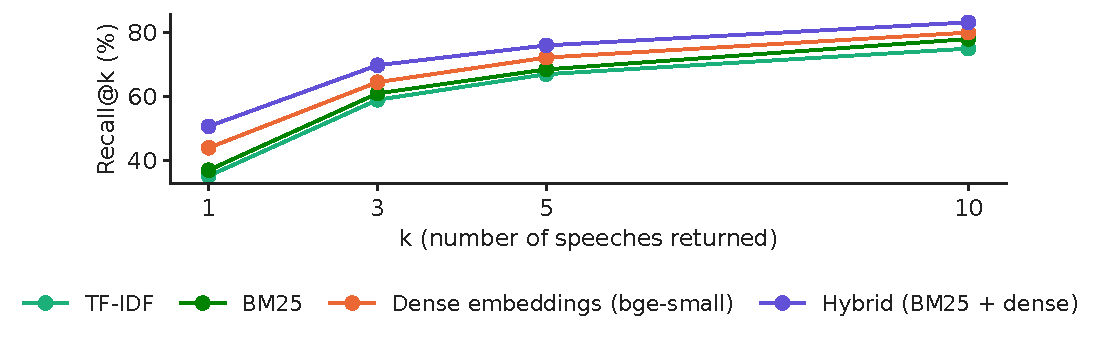
\includegraphics[width=\textwidth,height=0.500\textheight,keepaspectratio]{charts/en/rag_recall.pdf}\end{center}\vspace{-3mm}
\chartsource{Source: European Central Bank, speeches dataset. Data: 400 speeches, 8400 chunks; query = speech title.}
\vspace{0.5mm}
\begin{itemize}\setlength{\itemsep}{0pt}
  \item Recall@1: TF-IDF 35.2\,\%, BM25 37.0\,\%, dense 44.0\,\%, hybrid 50.7\,\%
    \begin{itemize}\setlength{\itemsep}{0pt}
      \item Recall@10 hybrid 83.2\,\%.
    \end{itemize}
\end{itemize}
\par\vfill\noindent{\scriptsize\color{FooterGray}}\hfill\qlink{NN\_L12\_rag\_recall}{Quantlets/L12/NN_L12_rag_recall}\par\vspace{0.5mm}
\end{frame}

\begin{frame}{Answers with and without retrieved documents}
\small
\intuition{question: which board member gave the speech with this title? 160 speeches since 15 Jan 2025, after the model's training data.}
\begin{center}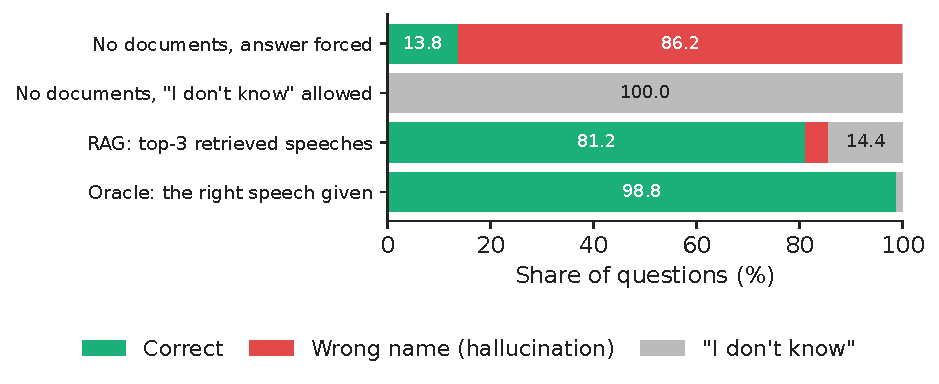
\includegraphics[width=\textwidth,height=0.350\textheight,keepaspectratio]{charts/en/rag_qa.pdf}\end{center}\vspace{-3mm}
\chartsource{Source: European Central Bank, speeches dataset. Data: 160 single-speaker speeches from 15 Jan 2025 to 30 Oct 2026; model Qwen2.5-3B-Instruct.}
\vspace{0.5mm}
\begin{itemize}\setlength{\itemsep}{0pt}
  \item Forced answer without documents: 86.2\,\% wrong names, Philip Lane 137 times
    \begin{itemize}\setlength{\itemsep}{0pt}
      \item RAG 81.2\,\% correct, oracle 98.8\,\%
      \item The most frequent speaker alone: 35.6\,\%.
    \end{itemize}
\end{itemize}
\par\vfill\manager{a confident wrong name is the costly failure: require sources in every answer and check them.}\par\vspace{0.5mm}
\par\vfill\noindent{\scriptsize\color{FooterGray}}\hfill\qlink{NN\_L12\_rag\_qa}{Quantlets/L12/NN_L12_rag_qa}\par\vspace{0.5mm}
\end{frame}

\begin{frame}{Design choices for a RAG system in a bank}
\small
\begin{itemize}\setlength{\itemsep}{3pt}
  \item \textbf{Chunking}
    \begin{itemize}\setlength{\itemsep}{0pt}
      \item 200 words with 50 overlap here; tables and footnotes need their own rules
    \end{itemize}
  \item \textbf{Metadata}
    \begin{itemize}\setlength{\itemsep}{0pt}
      \item Speaker, date and title travel with each chunk; the answer cites them
    \end{itemize}
  \item \textbf{Retriever}
    \begin{itemize}\setlength{\itemsep}{0pt}
      \item Hybrid BM25 + dense: recall@3 = 73.1\,\% on the question-answering speeches
    \end{itemize}
  \item \textbf{Abstention}
    \begin{itemize}\setlength{\itemsep}{0pt}
      \item Allow ``I don't know'': without documents the model then abstains on 100.0\,\% of questions
    \end{itemize}
  \item \textbf{Evaluation}
    \begin{itemize}\setlength{\itemsep}{0pt}
      \item A fixed set of questions with known answers, rerun after every change
    \end{itemize}
\end{itemize}
\end{frame}


\section{Language models as risk models: LLM-VaR}

\begin{frame}{LLM-VaR: a quantile forecast from the return history in the prompt}
\footnotesize
\intuition{no estimation and no fine-tuning: the model reads 250 returns and writes the Value-at-Risk (VaR).}
\begin{columns}[T,onlytextwidth]
\begin{column}{0.53\textwidth}
\[ \widehat{\mathrm{VaR}}^{\alpha}_{t+1}=\mathrm{LLM}\big(\mathrm{prompt}(r_{t-249},\dots,r_t;\alpha)\big) \]\[ \mathrm{LR}_{uc}=-2\ln\frac{(1-\alpha)^{n_0}\alpha^{n_1}}{(1-\hat\pi)^{n_0}\hat\pi^{n_1}}\sim\chi^2_1 \]{\footnotesize\begin{itemize}\setlength{\itemsep}{0pt}
  \item \textbf{\txtwhere}
    \begin{itemize}\setlength{\itemsep}{0pt}
      \item $r_t$ = daily log return of the S\&P 500 (\%)
      \item $\alpha\in\{1\,\%,5\,\%\}$
      \item Temperature 0
      \item $n_1$ = violations
      \item Kupiec likelihood ratio (LR) test.
    \end{itemize}
\end{itemize}\par}
\end{column}
\begin{column}{0.44\textwidth}
\begin{itemize}\setlength{\itemsep}{2pt}
  \item \textbf{Our replication}: Qwen2.5-3B-Instruct, 459 days from 2 Jan 2025 to 30 Oct 2026.
  \item \textbf{Benchmarks}: historical simulation (HS), 250 days
    \begin{itemize}\setlength{\itemsep}{0pt}
      \item Generalised autoregressive conditional heteroskedasticity (GARCH), GARCH(1,1)-$t$.
    \end{itemize}
\end{itemize}
\end{column}
\end{columns}
\par\vfill\manager{a 3B open model on a laptop is the cheapest test of the idea
    \begin{itemize}\setlength{\itemsep}{0pt}
      \item The paper used large commercial models.
    \end{itemize}}\par\vspace{0.5mm}
\par\vfill\noindent{\scriptsize\color{FooterGray}(Pele et al., 2026; Kupiec, 1995)}\hfill\tryit{notebook \S9}\par\vspace{0.5mm}
\end{frame}

\begin{frame}{LLM-VaR with a 3B open model on the S\&P 500}
\small
\intuition{the language model's 5\,\% VaR against GARCH; red dots mark the days the LLM-VaR was breached.}
\begin{center}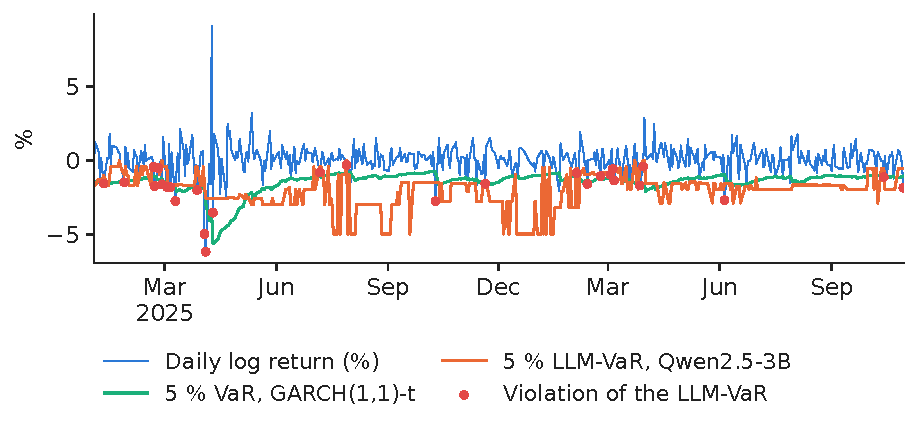
\includegraphics[width=\textwidth,height=0.476\textheight,keepaspectratio]{charts/en/llm_var.pdf}\end{center}\vspace{-3mm}
\chartsource{Source: Yahoo Finance, daily quotes. Data: 2 Jan 2025 to 30 Oct 2026, S\&P 500, trading days.}
\vspace{0.5mm}
\begin{itemize}\setlength{\itemsep}{0pt}
  \item 5\,\%: LLM 28 violations, GARCH 35, HS 23, expected 23.0.
  \item Mean 5\,\% VaR: LLM \ensuremath{-}1.99\,\%, GARCH \ensuremath{-}1.42\,\%
    \begin{itemize}\setlength{\itemsep}{0pt}
      \item Correlation of the two 0.05: the small model covers by being cautious, not by tracking volatility.
    \end{itemize}
\end{itemize}
\par\vfill\noindent{\scriptsize\color{FooterGray}}\hfill\qlink{NN\_L12\_llm\_var}{Quantlets/L12/NN_L12_llm_var}\par\vspace{0.5mm}
\end{frame}

\begin{frame}{Backtest of LLM-VaR against the classical benchmarks}
\small
{\footnotesize\renewcommand{\arraystretch}{1.05}\setlength{\tabcolsep}{4pt}
\begin{tabular}{@{}lrrrrrrr@{}}\toprule
Model & Viol.\ 1\,\% & Rate (\%) & $p_{uc}$ & Viol.\ 5\,\% & Rate (\%) & $p_{uc}$ & Mean VaR 5\,\% \\ \midrule
LLM-VaR (Qwen2.5-3B) & 4 & 0.87 & \cellcolor{Forest!55}0.777 & 28 & 6.10 & \cellcolor{Forest!55}0.295 & \ensuremath{-}1.99 \\
HS (250 days) & 6 & 1.31 & \cellcolor{Forest!55}0.528 & 23 & 5.01 & \cellcolor{Forest!55}0.991 & \ensuremath{-}1.56 \\
GARCH(1,1)-$t$ & 9 & 1.96 & \cellcolor{Forest!19}0.067 & 35 & 7.63 & \cellcolor{Crimson!37}0.016 & \ensuremath{-}1.42 \\
\bottomrule\end{tabular}}
\par\vspace{0.5mm}{\scriptsize \begin{itemize}\setlength{\itemsep}{0pt}
  \item Expected violations: 4.6 at 1\,\% and 23.0 at 5\,\%; green $p$-value: coverage not rejected at 10\,\%.
  \item Answers that could not be read as a number: 100.0\,\% parsed at 5\,\%, 100.0\,\% at 1\,\%; an unreadable answer keeps the previous day's value.
  \item Model size matters: the published study evaluated much larger models; results here describe a 3B model only.
\end{itemize}}
\par\vfill\noindent{\scriptsize\color{FooterGray}(own computation; Pele et al., 2026)}\hfill\tryit{notebook \S9}\par\vspace{0.5mm}
\end{frame}


\section{Risks and governance}

\begin{frame}{Six risks of LLMs in a financial institution, and the test for each}
\small
{\scriptsize\renewcommand{\arraystretch}{1.05}\setlength{\tabcolsep}{4pt}
\begin{tabular}{@{}p{0.2\textwidth}p{0.38\textwidth}p{0.36\textwidth}@{}}\toprule
Risk & Seen in this lecture & Control \\ \midrule
Hallucination & 86.2\,\% wrong speaker names without documents & RAG with sources; abstention allowed \\
Leakage / contamination & lower perplexity on older speeches & test on text after the cut-off \\
Prompt sensitivity & 12.9 macro-F1 points across wordings & select on validation, freeze, version \\
Miscalibration & ECE 4.7\,\% zero-shot, 5.4\,\% TF-IDF & temperature scaling, thresholds on validation \\
Cost and latency & 389 ms vs 2.50 ms per sentence & smallest model that passes the test \\
Data protection & client documents in prompts & local models; duties of the European Union (EU) Artificial Intelligence (AI) Act for high-risk uses such as credit scoring \\
\bottomrule\end{tabular}}
\par\vspace{0.5mm}{\scriptsize \begin{itemize}\setlength{\itemsep}{0pt}
  \item The EU AI Act is Regulation (EU) 2024/1689.
\end{itemize}}
\end{frame}

\section*{Wrap-up}

\begin{frame}{Quiz 1: temperature}
\small
\begin{itemize}
  \item You classify 10,000 news items with an LLM and get different labels on two runs of the same item
    \begin{itemize}\setlength{\itemsep}{0pt}
      \item What do you change first?
    \end{itemize}
\end{itemize}
\vspace{2mm}
\begin{exampleblock}{Answer}
\begin{itemize}
  \item Set temperature to 0 (or read label probabilities): sampling at $T>0$ is random by construction.
\end{itemize}
\end{exampleblock}
\end{frame}

\begin{frame}{Quiz 2: evaluation}
\small
\begin{itemize}
  \item A vendor reports 95\,\% accuracy of its LLM on Financial PhraseBank
    \begin{itemize}\setlength{\itemsep}{0pt}
      \item What two questions do you ask?
    \end{itemize}
\end{itemize}
\vspace{2mm}
\begin{exampleblock}{Answer}
\begin{itemize}
  \item Which agreement subset (the unanimous one is easiest) and was PhraseBank in the training data (published 2014, widely copied)? Ask for macro-F1 too: 61.4\,\% of the sentences are neutral.
\end{itemize}
\end{exampleblock}
\end{frame}

\begin{frame}{Quiz 3: RAG}
\small
\begin{itemize}
  \item Your RAG assistant answers wrongly although the right document exists in the corpus
    \begin{itemize}\setlength{\itemsep}{0pt}
      \item Where do you look first?
    \end{itemize}
\end{itemize}
\vspace{2mm}
\begin{exampleblock}{Answer}
\begin{itemize}
  \item At the retriever: check whether the document is in the top $k$ (recall@k)
    \begin{itemize}\setlength{\itemsep}{0pt}
      \item Only then at the prompt and the model.
    \end{itemize}
\end{itemize}
\end{exampleblock}
\end{frame}

\begin{frame}{Wrap-up}
\small
\begin{itemize}\setlength{\itemsep}{4pt}
  \item An LLM is a next-token model
    \begin{itemize}\setlength{\itemsep}{0pt}
      \item Perplexity, temperature and tokens are its basic quantities.
    \end{itemize}
  \item A prompt is a model: score it on held-out labels, with intervals, seeds and paraphrases.
  \item With labels, small trained models and LLM embeddings are hard to beat
    \begin{itemize}\setlength{\itemsep}{0pt}
      \item Without labels, prompting gives a strong start.
    \end{itemize}
  \item RAG turns hallucinated answers into sourced ones
    \begin{itemize}\setlength{\itemsep}{0pt}
      \item Evaluate the retriever first.
    \end{itemize}
  \item Next: time-series foundation models for energy and finance (Lecture 13).
\end{itemize}
\end{frame}

\begin{frame}{Research from our group}
\footnotesize
\begin{itemize}\setlength{\itemsep}{4pt}
  \item \textbf{LLM-VaR and, for the expected shortfall (ES), LLM-ES}: general-purpose LLMs estimate both risk measures zero-shot from a structured prompt with past returns
    \begin{itemize}\setlength{\itemsep}{0pt}
      \item Backtested against classical risk models (Pele, Bolovăneanu, Lin, Ren, Ginavar, Spilak, Andrei, Toma, Lessmann \& Härdle, 2026, Expert Systems with Applications).
    \end{itemize}
  \item \textbf{LLM-driven stock prediction}: LLaMA 3.3 combines price history with news sentiment in the prompt and outperforms LLaMA 3.1 and an autoregressive integrated moving-average benchmark (Tak \& Pele, 2025, PICBE).
  \item \textbf{Central-bank narratives}: a transformer-based sentiment index of the National Bank of Romania's minutes improves Romanian inflation forecasts (Amza, Bolovăneanu \& Pele, 2026, PICBE) --- the same kind of text as our ECB speeches.
\end{itemize}
\par\vspace{0.5mm}{\scriptsize \begin{itemize}\setlength{\itemsep}{0pt}
  \item Findings as stated in the papers' abstracts; numbers on the other slides come from our own data.
\end{itemize}}
\par\vfill\noindent{\scriptsize\color{FooterGray}(Bucharest University of Economic Studies, ASE; Romanian Academy, Institute for Economic Forecasting, IPE)}\par\vspace{0.5mm}
\end{frame}

\begin{frame}{Further reading and resources}
\small
\begin{columns}[T,onlytextwidth]
\begin{column}{0.5\textwidth}
\begin{itemize}\setlength{\itemsep}{4pt}
  \item \textbf{Hugging Face} course on LLMs: \href{https://huggingface.co/learn/llm-course}{huggingface.co/learn/llm-course}.
  \item \textbf{Qwen2.5} models and report: \href{https://huggingface.co/Qwen}{huggingface.co/Qwen}.
  \item \textbf{Prompting guide}: \href{https://www.promptingguide.ai}{promptingguide.ai}.
\end{itemize}
\end{column}
\begin{column}{0.47\textwidth}
\begin{itemize}\setlength{\itemsep}{4pt}
  \item \textbf{ECB speeches} data set: \href{https://www.ecb.europa.eu/press/key/html/downloads.en.html}{ecb.europa.eu}.
  \item \textbf{Quantinar}: The Next Word Problem: \href{https://quantinar.com/course/100100/the-next-word-problem-full-course}{quantinar.com}.
  \item \textbf{This lecture}: notebook, seminar and Quantlets --- \href{https://github.com/danpele/NEURAL_BIZ}{github.com/danpele/NEURAL\_BIZ}.
\end{itemize}
\end{column}
\end{columns}
\end{frame}

\begin{frame}{References (1/2)}
\scriptsize
\begin{itemize}\setlength{\itemsep}{0pt}\scriptsize
\item Amza, A., Bolovăneanu, V.\ \& Pele, D.\,T.\ (2026). Inflation forecasting with monetary policy narratives: Evidence from an emerging economy. \textit{Proceedings of the International Conference on Business Excellence}, 20(1), 75--83. \href{https://doi.org/10.2478/picbe-2026-0012}{doi:10.2478/picbe-2026-0012}
\item Brown, T.\,B.\ et al.\ (2020). Language models are few-shot learners. \textit{Advances in Neural Information Processing Systems}, 33. \href{https://arxiv.org/abs/2005.14165}{arXiv:2005.14165}
\item Guo, C., Pleiss, G., Sun, Y.\ \& Weinberger, K.\,Q.\ (2017). On calibration of modern neural networks. \textit{Proceedings of the 34th International Conference on Machine Learning}, 1321--1330. \href{https://arxiv.org/abs/1706.04599}{arXiv:1706.04599}
\item Hoffmann, J.\ et al.\ (2022). Training compute-optimal large language models. \textit{Advances in Neural Information Processing Systems}, 35. \href{https://arxiv.org/abs/2203.15556}{arXiv:2203.15556}
\item Hu, E.\,J., Shen, Y., Wallis, P., Allen-Zhu, Z., Li, Y., Wang, S., Wang, L.\ \& Chen, W.\ (2022). LoRA: Low-rank adaptation of large language models. \textit{International Conference on Learning Representations}. \href{https://arxiv.org/abs/2106.09685}{arXiv:2106.09685}
\item Kaplan, J.\ et al.\ (2020). Scaling laws for neural language models. \href{https://arxiv.org/abs/2001.08361}{arXiv:2001.08361}
\item Kupiec, P.\,H.\ (1995). Techniques for verifying the accuracy of risk measurement models. \textit{The Journal of Derivatives}, 3(2), 73--84. \href{https://doi.org/10.3905/jod.1995.407942}{doi:10.3905/jod.1995.407942}
\item Lewis, P.\ et al.\ (2020). Retrieval-augmented generation for knowledge-intensive NLP tasks. \textit{Advances in Neural Information Processing Systems}, 33. \href{https://arxiv.org/abs/2005.11401}{arXiv:2005.11401}
\item Malo, P., Sinha, A., Korhonen, P., Wallenius, J.\ \& Takala, P.\ (2014). Good debt or bad debt: Detecting semantic orientations in economic texts. \textit{Journal of the Association for Information Science and Technology}, 65(4), 782--796. \href{https://doi.org/10.1002/asi.23062}{doi:10.1002/asi.23062}
\item Ouyang, L.\ et al.\ (2022). Training language models to follow instructions with human feedback. \textit{Advances in Neural Information Processing Systems}, 35. \href{https://arxiv.org/abs/2203.02155}{arXiv:2203.02155}
\end{itemize}
\end{frame}

\begin{frame}{References (2/2)}
\scriptsize
\begin{itemize}\setlength{\itemsep}{0pt}\scriptsize
\item Pele, D.\,T., Bolovăneanu, V., Lin, M.-B., Ren, R., Ginavar, A.\,T., Spilak, B., Andrei, A.-V., Toma, F.-M., Lessmann, S.\ \& Härdle, W.\,K.\ (2026). In the beginning was the Word: LLM-VaR and LLM-ES. \textit{Expert Systems with Applications}, 295, 128676. \href{https://doi.org/10.1016/j.eswa.2025.128676}{doi:10.1016/j.eswa.2025.128676}
\item Qwen Team (2024). Qwen2.5 technical report. \href{https://arxiv.org/abs/2412.15115}{arXiv:2412.15115}
\item Rafailov, R., Sharma, A., Mitchell, E., Ermon, S., Manning, C.\,D.\ \& Finn, C.\ (2023). Direct preference optimization: Your language model is secretly a reward model. \textit{Advances in Neural Information Processing Systems}, 36. \href{https://arxiv.org/abs/2305.18290}{arXiv:2305.18290}
\item Robertson, S.\ \& Zaragoza, H.\ (2009). The probabilistic relevance framework: BM25 and beyond. \textit{Foundations and Trends in Information Retrieval}, 3(4), 333--389. \href{https://doi.org/10.1561/1500000019}{doi:10.1561/1500000019}
\item Sennrich, R., Haddow, B.\ \& Birch, A.\ (2016). Neural machine translation of rare words with subword units. \textit{Proceedings of the 54th Annual Meeting of the ACL}, 1715--1725. \href{https://doi.org/10.18653/v1/P16-1162}{doi:10.18653/v1/P16-1162}
\item Tak, R.\ \& Pele, D.\,T.\ (2025). LLM-driven stock prediction: Capturing market trends with LLaMA. \textit{Proceedings of the International Conference on Business Excellence}, 19(1), 529--540. \href{https://doi.org/10.2478/picbe-2025-0043}{doi:10.2478/picbe-2025-0043}
\item Wei, J.\ et al.\ (2022). Chain-of-thought prompting elicits reasoning in large language models. \textit{Advances in Neural Information Processing Systems}, 35. \href{https://arxiv.org/abs/2201.11903}{arXiv:2201.11903}
\item Xiao, S., Liu, Z., Zhang, P.\ \& Muennighoff, N.\ (2023). C-Pack: Packaged resources to advance general Chinese embedding (BAAI general embedding). \href{https://arxiv.org/abs/2309.07597}{arXiv:2309.07597}
\item Zhao, Z., Wallace, E., Feng, S., Klein, D.\ \& Singh, S.\ (2021). Calibrate before use: Improving few-shot performance of language models. \textit{Proceedings of the 38th International Conference on Machine Learning}, 12697--12706. \href{https://arxiv.org/abs/2102.09690}{arXiv:2102.09690}
\end{itemize}
\end{frame}

\appendix

\section*{Appendix}

\begin{frame}{Appendix A: the prompt used for zero-shot classification}
\small
\begin{itemize}\setlength{\itemsep}{4pt}
  \item \textbf{System}
    \begin{itemize}\setlength{\itemsep}{0pt}
      \item ``You are a careful financial analyst.''
    \end{itemize}
  \item \textbf{User}
    \begin{itemize}\setlength{\itemsep}{0pt}
      \item ``Classify the sentiment of this sentence from financial news, from the point of view of an investor in the company. Answer with one word: positive, negative or neutral. Sentence: \ldots{} Answer:''
    \end{itemize}
  \item \textbf{Few-shot}
    \begin{itemize}\setlength{\itemsep}{0pt}
      \item The same, with ``Sentence: \ldots{} Answer: label'' pairs before the input; examples balanced across classes and shuffled
    \end{itemize}
  \item \textbf{Chain-of-thought}
    \begin{itemize}\setlength{\itemsep}{0pt}
      \item ``\ldots{} First explain your reasoning in at most two short sentences, then give the final answer on a new line as `Label: <positive|negative|neutral>'.''
    \end{itemize}
\end{itemize}
\end{frame}

\begin{frame}{Appendix B: implementation details}
\small
\begin{itemize}\setlength{\itemsep}{4pt}
  \item Models in float16 on the laptop's graphics processor (PyTorch)
    \begin{itemize}\setlength{\itemsep}{0pt}
      \item Hugging Face transformers
      \item Scikit-learn for TF-IDF, logistic regression and bootstrap.
    \end{itemize}
  \item Seeds: 20261108 for splits and samples
    \begin{itemize}\setlength{\itemsep}{0pt}
      \item Few-shot examples drawn with seeds 20261108, +1 and +2.
    \end{itemize}
  \item The whole analysis took 2.2 minutes on its last run (model outputs cached)
    \begin{itemize}\setlength{\itemsep}{0pt}
      \item First run about 40 minutes.
    \end{itemize}
  \item Per-item predictions are published with the Quantlets, so every number can be recomputed without a graphics card.
\end{itemize}
\end{frame}

\end{document}
